\documentclass[11pt,dvipdfmx]{jreport}
\usepackage{wuse_thesis}
\usepackage{indentfirst}
\usepackage{url}	% \url{}コマンド用.URLを表示する際に便利
\usepackage{graphicx}  % ←graphicx.styを用いてEPSを取り込む場合有効にする
\usepackage{listings,jvlisting} %日本語のコメントアウトをする場合jvlisting(もしくはjlisting)が必要

\usepackage{multirow}

\usepackage{color}

\renewcommand{\lstlistingname}{Program}
\newcommand{\todo}[1]{\colorbox{yellow}{{\bf TODO}:}{\color{red} {\textbf{[#1]}}}}
			% 他のパッケージ・スタイルを使う場合には適宜追加

%ここからソースコードの表示に関する設定
\definecolor{darkgray}{rgb}{.4,.4,.4}
\definecolor{purple}{rgb}{0.65, 0.12, 0.82}

\lstdefinelanguage{JavaScript}{
  keywords={typeof, new, true, false, catch, function, return, null, catch, switch, var, if, in, while, do, else, case, break},
  keywordstyle=\color{blue}\bfseries,
  ndkeywords={class, export, boolean, throw, implements, import, this},
  ndkeywordstyle=\color{darkgray}\bfseries,
  identifierstyle=\color{black},
  sensitive=false,
  comment=[l]{//},
  morecomment=[s]{/*}{*/},
  commentstyle=\color{purple}\ttfamily,
  stringstyle={\small\ttfamily},
  morestring=[b]',
  morestring=[b]"
}

\lstset{
  basicstyle={\ttfamily},
  identifierstyle={\small},
  commentstyle={\smallitshape},
  keywordstyle={\small\bfseries},
  ndkeywordstyle={\small},
  stringstyle={\small\ttfamily},
  frame={tb},
  breaklines=true,
  columns=[l]{fullflexible},
  numbers=left,
  xrightmargin=0zw,
  xleftmargin=3zw,
  numberstyle={\scriptsize},
  stepnumber=1,
  numbersep=1zw,
  lineskip=-0.5ex
}
%ここまでソースコードの表示に関する設定

%%%%%%%%%%%%%%%%%%%%%%%%%%%%%%%%%%%%%%%%%%%%%%%%%%%%%%%%%%%%%%%%%%%%%%%%

%%%%%%%%%%%%%%%%%%%%%%%%%%%%%%%%%%%%%%%%%%%%%%%%%%%%%%%%%%%%%%%%%%%%%%%%

%%
%% 主に表紙を作成するための情報
%%

%%  タイトル(修論の場合は英語表記も指定)
\title{JavaScriptライブラリのテストコード変更内容に基づく後方互換性損失の検出}
%\etitle{Test\\Test\\Test}

%%  著者名(修論の場合は英語表記も指定)
\author{前川 大樹}
%\eauthor{Akinori Ihara}

%% 卒業論文・修士論文(以下のどちらかを選択)
\bachelar	% 卒業論文(4年生用)
%\master  	% 修士論文(M2用)

%%  学科・クラスタ
\department{システム工}
%\department{デザイン情報}
%\department{デザイン科学}

%%  学生番号
\studentid{60256245}

%%  卒業年度
\gyear{2023}		% 提出年が2022年なら,2021年度

%%  論文提出日
\date{2024年2月13日}	% 修士の場合は月(2021年2月)までとし,英語表記も指定
%\edate{February 2021}	% 修士の場合,こちら(英語表記)も有効化

%%%%%%%%%%%%%%%%%%%%%%%%%%%%%%%%%%%%%%%%%%%%%%%%%%%%%%%%%%%%%%%%%%%%%%%%

\begin{document}

\maketitle

%%
%%  概要
%%
\begin{abstract}
本研究では,ソフトウェアの後方互換性の損失をテストコードの変更内容に基づいて判定する手法を提案する.

ソフトウェア開発では,ライブラリと呼ばれる再利用可能なプログラムの利用により,開発者自身が同じ機能を再実装する必要がなくなり開発効率が向上する.ライブラリに対して行われる変更は,軽微な修正であっても破壊的変更が含まれることがあり,変更後のライブラリが後方互換性を維持しているか否かをライブラリ利用者が正確に判断することは困難である.

従来研究では,ライブラリの動作を検証するテストコードの変更有無に着目した後方互換性の損失の検出手法を提案している.しかし,テストコードはテストケースの実行手順の変更など,ライブラリの変更とは無関係に変更されることがあり,従来手法ではテストコードの変更内容は考慮されておらず誤検出が多い.

本研究では,テストコードの変更内容を詳細に分析することで,後方互換性の損失をより正確に検出することを目指す.具体的には,後方互換性が損失するライブラリバージョンにおけるテストコードの変更内容を明らかにし,自動検出するツールを開発して後方互換性の損失の検出精度を検証する.

\end{abstract}

%%  目次
\tableofcontents

%%  図目次 (図目次をいれたければ以下のコメントをはずす)
%\listoffigures

%%  表目次 (表目次をいれたければ以下のコメントをはずす)
%\listoftables

\newpage
\pagenumbering{arabic}	% 以降のページ番号を算用数字に

%%%%%%%%%%%%%%%%%%%%%%%%%%%%%%%%%%%%%%%%%%%%%%%%%%%%%%%%%%%%%%%%%%%%%%%%

%%
%%  本文はここから
%%

\chapter{はじめに}
ソフトウェア開発では,ライブラリと呼ばれる再利用可能なプログラムの利用により,開発者自身が同じ機能を再実装する必要がなくなり開発効率が向上する\cite{shared-software}\cite{effect-on-developer}.ソフトウェアは新機能の追加,バグ修正などによって頻繁に更新されており,ライブラリも例外ではない\cite{library-analysis}.ライブラリの更新には,脆弱性の修正などライブラリの利用者であるクライアントにとって重要な変更が含まれることがあり,これによりクライアントは依存ライブラリの更新を余儀なくされることも多い.クライアント開発者が依存ライブラリを更新する際,更新後ライブラリに機能削除や仕様変更といったクライアントに影響を与える変更が含まれる場合,更新前の仕様を前提とするクライアントと,更新後ライブラリのソースコードに不整合が生じ,クライアントソフトウェアがエラーになってしまうことがある.このような,更新後のライブラリがクライアントに影響を与えることを後方互換性を損失するという.ライブラリ開発者はクライアントに影響を与えないよう,ライブラリの後方互換性の有無をクライアントに正確に伝えることが求められる.

ライブラリ開発者が更新後ライブラリの後方互換性の有無をクライアントに伝える手法として,セマンティックバージョニング\footnote{\url{https://semver.org}}がある.セマンティックバージョニングは,ライブラリ開発者がライブラリにバージョン名を付与するための規則で,バージョン名を「1.0.0」などの3つの数字で表す.それぞれの数字は,「メジャー.マイナー.パッチ」と呼ばれ,後方互換性を損失する変更ではメジャー,後方互換性を維持する変更ではマイナー,またはパッチの値を増やし新しいバージョン名を付与する.しかし,バージョン名の付与はライブラリ開発者が手動で行うため,後方互換性を損失しているにも関わらず誤ってマイナーやパッチに分類されてしまうことがある.Javaのような静的型付け言語では,バージョニングシステムを使用しなくても型情報が後方互換性の損失を判断することに役立つ.例えば,ライブラリのメソッドの型が変更された場合,当該メソッドを利用するクライアントコードはコンパイルできなくなる.一方JavaScriptなどの動的型付け言語では,型情報やコンパイルがないため,誤ったバージョン名による影響はクライアントソフトウェアの実行時まで検出されないことが多い.この課題に対して,JavaScriptライブラリの後方互換性の損失を検出する研究が行われている.

松田らは,後方互換性を損失するライブラリの更新は,プログラムの更新と合わせてテストコードも修正すると考え,テストコードの変更有無による後方互換性損失の検出手法を提案した\cite{matsuda}.しかし,テストコードの変更内容を考慮しておらず,テストコードの実行手順の修正のようなライブラリの更新とは無関係のテストコード変更についても後方互換性を損失したと誤検出する.本研究では,テストコードの変更内容を詳細に分析することで,後方互換性の損失をより正確に検出することを目指す.具体的には,2つのResearch Question(RQ)に回答する.

\begin{itemize}
  \item RQ1:後方互換性の損失に伴うテストコード変更とは何か?
  \item RQ2:テストコード変更内容に基づく後方互換性損失の検出手法の有効性はどの程度か?
\end{itemize}

RQ1では,ライブラリ更新が後方互換性の損失を含む際,それに伴ってどのようなテストコード変更が行われているかを分析し,後方互換性の損失を検出する手がかりとなるテストコード変更内容を明らかにする.RQ2では,これらの変更内容を自動検出するツールを開発し,後方互換性損失の検出精度を検証する.

以降,本論文では,\ref{chap:backward-compatibility}章で後方互換性の損失がクライアントソフトウェアに与える影響と関連研究,本研究の位置付けを述べ,\ref{chap:rq1}章,\ref{chap:rq2}章では,設定したRQにおけるそれぞれの分析手法,結果,考察を述べる.続く\ref{chap:heuristic}章では,妥当性の脅威を述べ,最後に\ref{chap:end}章で本論文をまとめる.

\chapter{後方互換性の損失}\label{chap:backward-compatibility}

\section{後方互換性の損失の原因}
ライブラリが後方互換性を損失する原因として,ライブラリが提供するAPI(アプリケーションプログラミングインターフェース)の振る舞いの変更がある.メソッド,シグネチャ,例外,入出力データ形式など,APIの振る舞いの変更は全てクライアントに影響を与える可能性がある.APIの機能拡張やバグ修正であっても,拡張された機能が存在しないことや,壊れている動作に依存していた場合,クライアントソフトウェアにエラーを引き起こす原因になる.一方,提供するAPIの追加や,ライブラリの内部でのみ使用されるモジュールの変更は一般的にクライアントは影響を受けない.Java言語では,privateアクセス修飾子等を利用することで,クライアントに影響を与えることなく内部でのみ利用するモジュールを変更することができる.しかし,JavaScript言語ではライブラリのどのモジュールをAPIとしてクライアントに提供し,どのモジュールを内部で使用するかが明確に定義されることが少なく,ライブラリ開発者が内部使用のみを意図してモジュールの振る舞いを変更しても,多数のクライアントが当該モジュールを使用しており影響を受けることもある.例として,ユーザインターフェースを構築するReactというライブラリの15.3.2から15.4.0へのマイナーアップデート\footnote{\url{https://github.com/facebook/react/compare/v15.3.2...v15.4.0}}を挙げる.この変更では,react/lib/ReactMountモジュールを刷新する変更が行われた.ライブラリ開発者は,内部使用のみを意図していたが,多数のクライアントが当該モジュールを使用しており,影響を受けた\footnote{\url{https://github.com/rekit/rekit/issues/16}}

\section{クライアントソフトウェアに与える影響}
JavaScriptライブラリの後方互換性の損失がクライアントソフトウェアに与える影響を調査した研究\cite{impact-analysis-for-clients}では,npm\footnote{\url{https://www.npmjs.com/}}から384件のクライアントソフトウェアを調査し,11.7%が後方互換性の損失の影響を受けたことが示されている.また,後方互換性損失の約44%が,ライブラリのマイナーリリースとパッチリリースであったことも示されており,ライブラリ開発者にとってバージョン名を適切に付与することは難しいとわかる.ライブラリのバージョン名に誤った値が付与されている場合,クライアント開発者が後方互換性を維持することを期待してライブラリバージョンを適用し,エラーが引き起こされてしまうことになる.例として,2016年12月,デバック用のAPIを提供するdebugというライブラリの2.3.3から2.4.0へのマイナーアップデート\footnote{\url{https://github.com/debug-js/debug/compare/2.3.3...2.4.0}}では,単純なスペルミスによるバグが混入し\footnote{\url{https://github.com/debug-js/debug/issues/347}},新バージョンを適用しようとしたクライアントソフトウェアはエラーを引き起こした.バグは1時間以内に修正されたが\footnote{\url{https://github.com/debug-js/debug/pull/356}},debugは12月だけでも2,700万回以上ダウンロードされ,多数のクライアントが影響を受けた.

\section{関連研究}
ライブラリ開発者が誤ったバージョン名を付与し,クライアントにエラーを引き起こすことを防ぐため,JavaScript言語における後方互換性の損失を検出する研究が行われている.

Møllerらは,クライアント開発者がクライアントの動作を検証するために作成したテスト(以降,クライアントテスト)を利用し,動的型付け言語であるJavaScriptの型情報をクライアントテストによって補うことで後方互換性の損失の検出を試みた\cite{type-regression-testing}\cite{model-based-testing}.本研究では,クライアントテストといったライブラリ外の資源は利用せず,ライブラリに付属するテストのみから後方互換性の損失を検出する手法を提案する.

Kraaijeveldは,後方互換性を損失する変更を,ライブラリが定義している関数名やパラメータ数の変更と定義し,後方互換性の損失の検出を試みた\cite{detecting-breaking-changes-in-js-apis}.ただし,この手法では関数やクラスの入出力形式の変更や,例外処理の追加などによる後方互換性の損失を検出することができない.本研究では,ライブラリの動作を検証するテストコードを利用する.テストコードは,テスト対象となる関数やクラスの入出力の情報や例外の情報を有しており,ライブラリの後方互換性の損失の種類を絞ることなく検出することを目指す.

\section{先行研究}
関連研究が示すとおり,動的型付け言語であるJavaScript言語における後方互換性の損失の検出は多くの場合に困難である.

松田らは,JavaScriptライブラリに付属するテストコードが,テスト対象となる関数やクラスの入出力の情報を含んでおり,型情報を補うことができる点に着目し,ライブラリのテストコード変更有無に基づく後方互換性の検出手法を提案した\cite{matsuda}(以降,従来手法).ライブラリが更新される際,その動作を検証するテストコードも通常更新される.したがって,テストコードの変更有無から後方互換性の損失を検出できる場合がある.従来手法は,テストコードをテストケースの追加,変更,削除,変更なしに分類し,テストケースの変更・削除に対して後方互換性を損失したと検出する.ただし,APIの仕様変更に伴って,新しい仕様をカバーするためにテストケースが追加されることや,テストの実行手順の修正や可読性向上のためのフォーマッティングなど,プログラムの変更とは無関係にテストコードが変更されることも考えられ,そのような変更は誤検出の原因になる.

\section{キーアイデア}\label{sec:key-idea}
従来手法では,テストコードの変更を4つに分類することで後方互換性損失の検出を試みたが誤検出が多い結果となった.本研究では,後方互換性を損失するライブラリ変更に伴うテストコード変更には特徴があると考え,テストコード変更内容に基づく後方互換性の損失の検出手法を提案し精度を検証する.

図\ref{fig:motivation}は,後方互換性の損失に伴うテストコード変更の例として,JavaScriptオブジェクトを文字列に変換する関数を提供するライブラリserialize-javascriptのバージョン2.1.0から2.1.1へのパッチアップデート\footnote{\url{https://github.com/yahoo/serialize-javascript/compare/v2.1.0...v2.1.1}}を示す.上部がソースコード,下部がテストコード変更内容である.ソースコードの191行目で,190行目の条件に合致する特定の入力に対する関数の返り値が変更されている.この変更に伴って,対応するテストコードも修正されている.テストコードの254行目の変更では,テスト対象となる関数とパラメータはそのままで,期待する返り値のみ変更されている.このように,テストコードの変更内容には特徴があるため,テストコードの変更内容をより詳細に分析することで,後方互換性の損失を正確に検出することを目指す.

\begin{figure}[t]
  \label{fig:motivation}
  \centering
  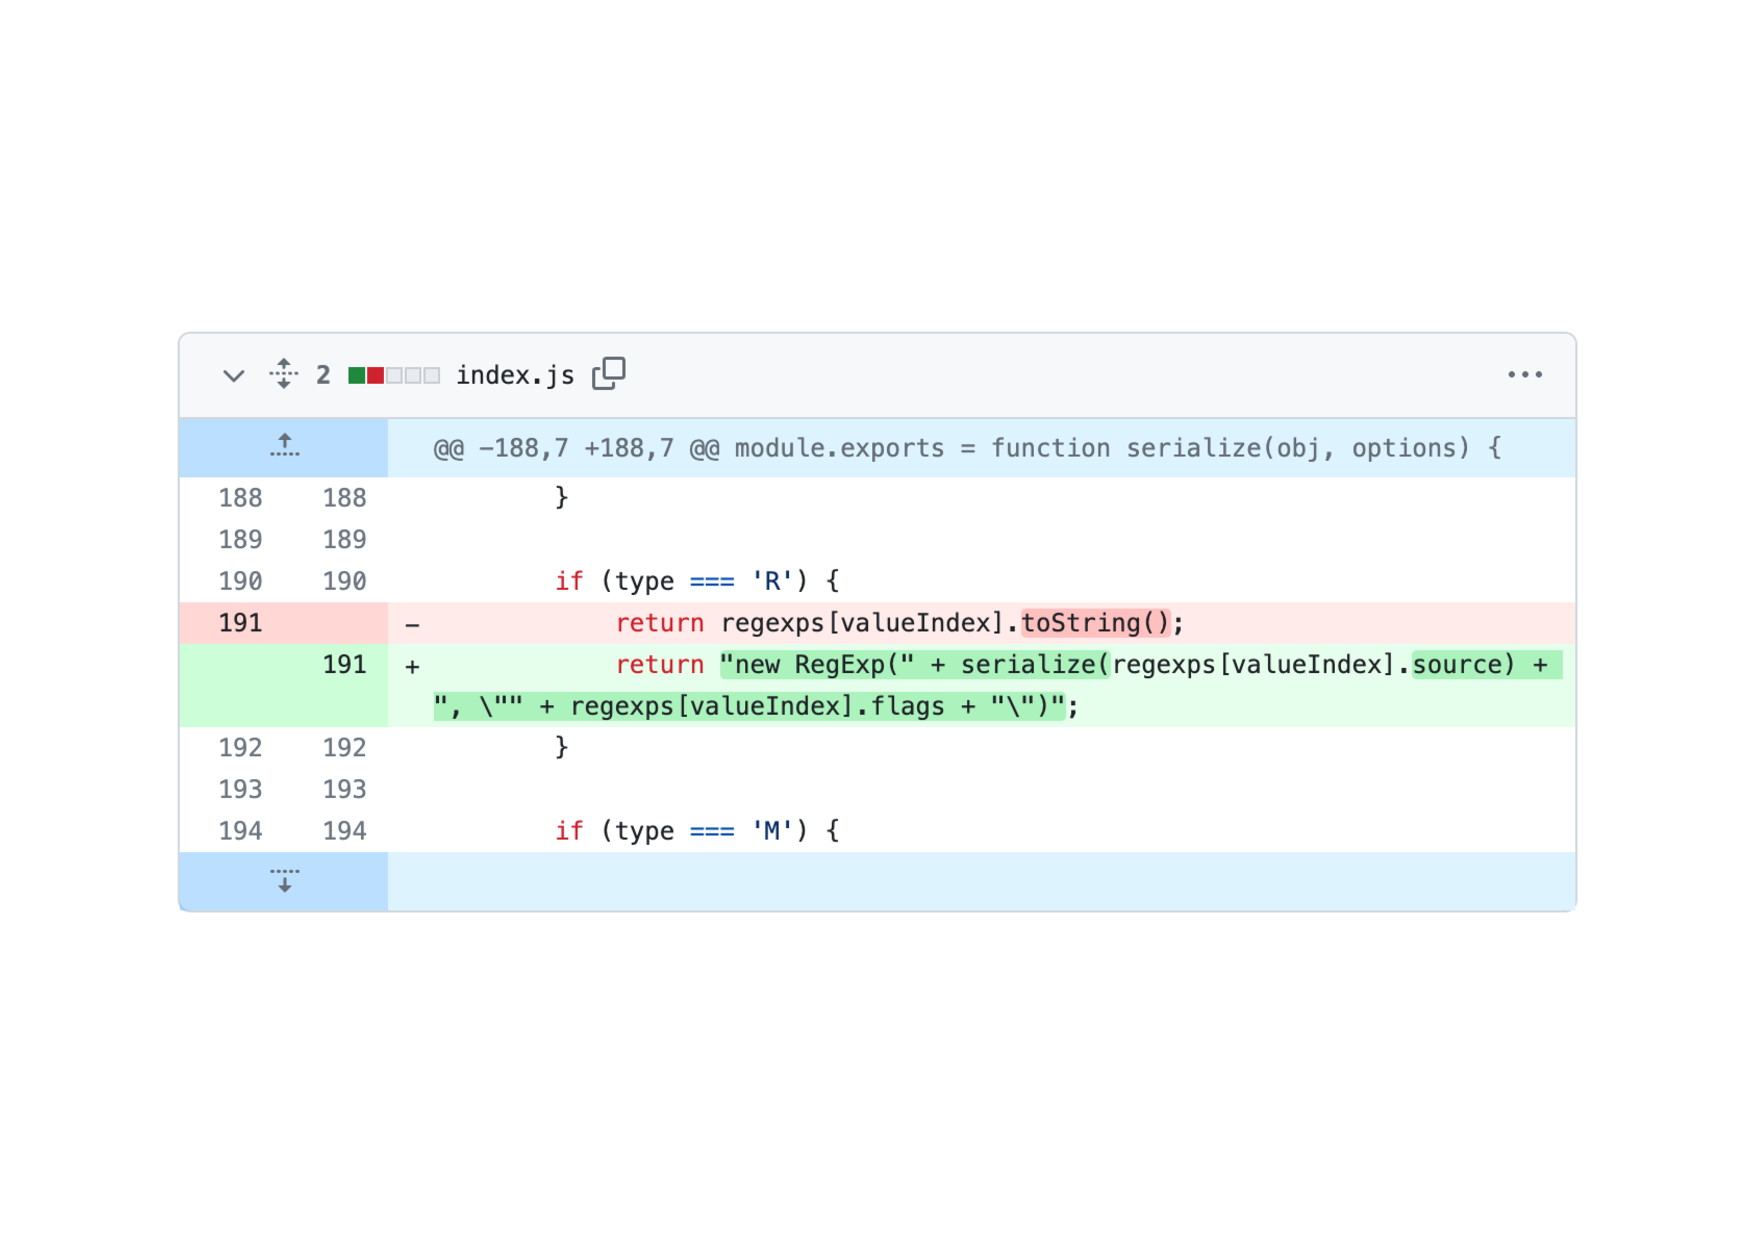
\includegraphics[width=1.0\linewidth]{fig/rq1/serialize-javascript/index.pdf}
  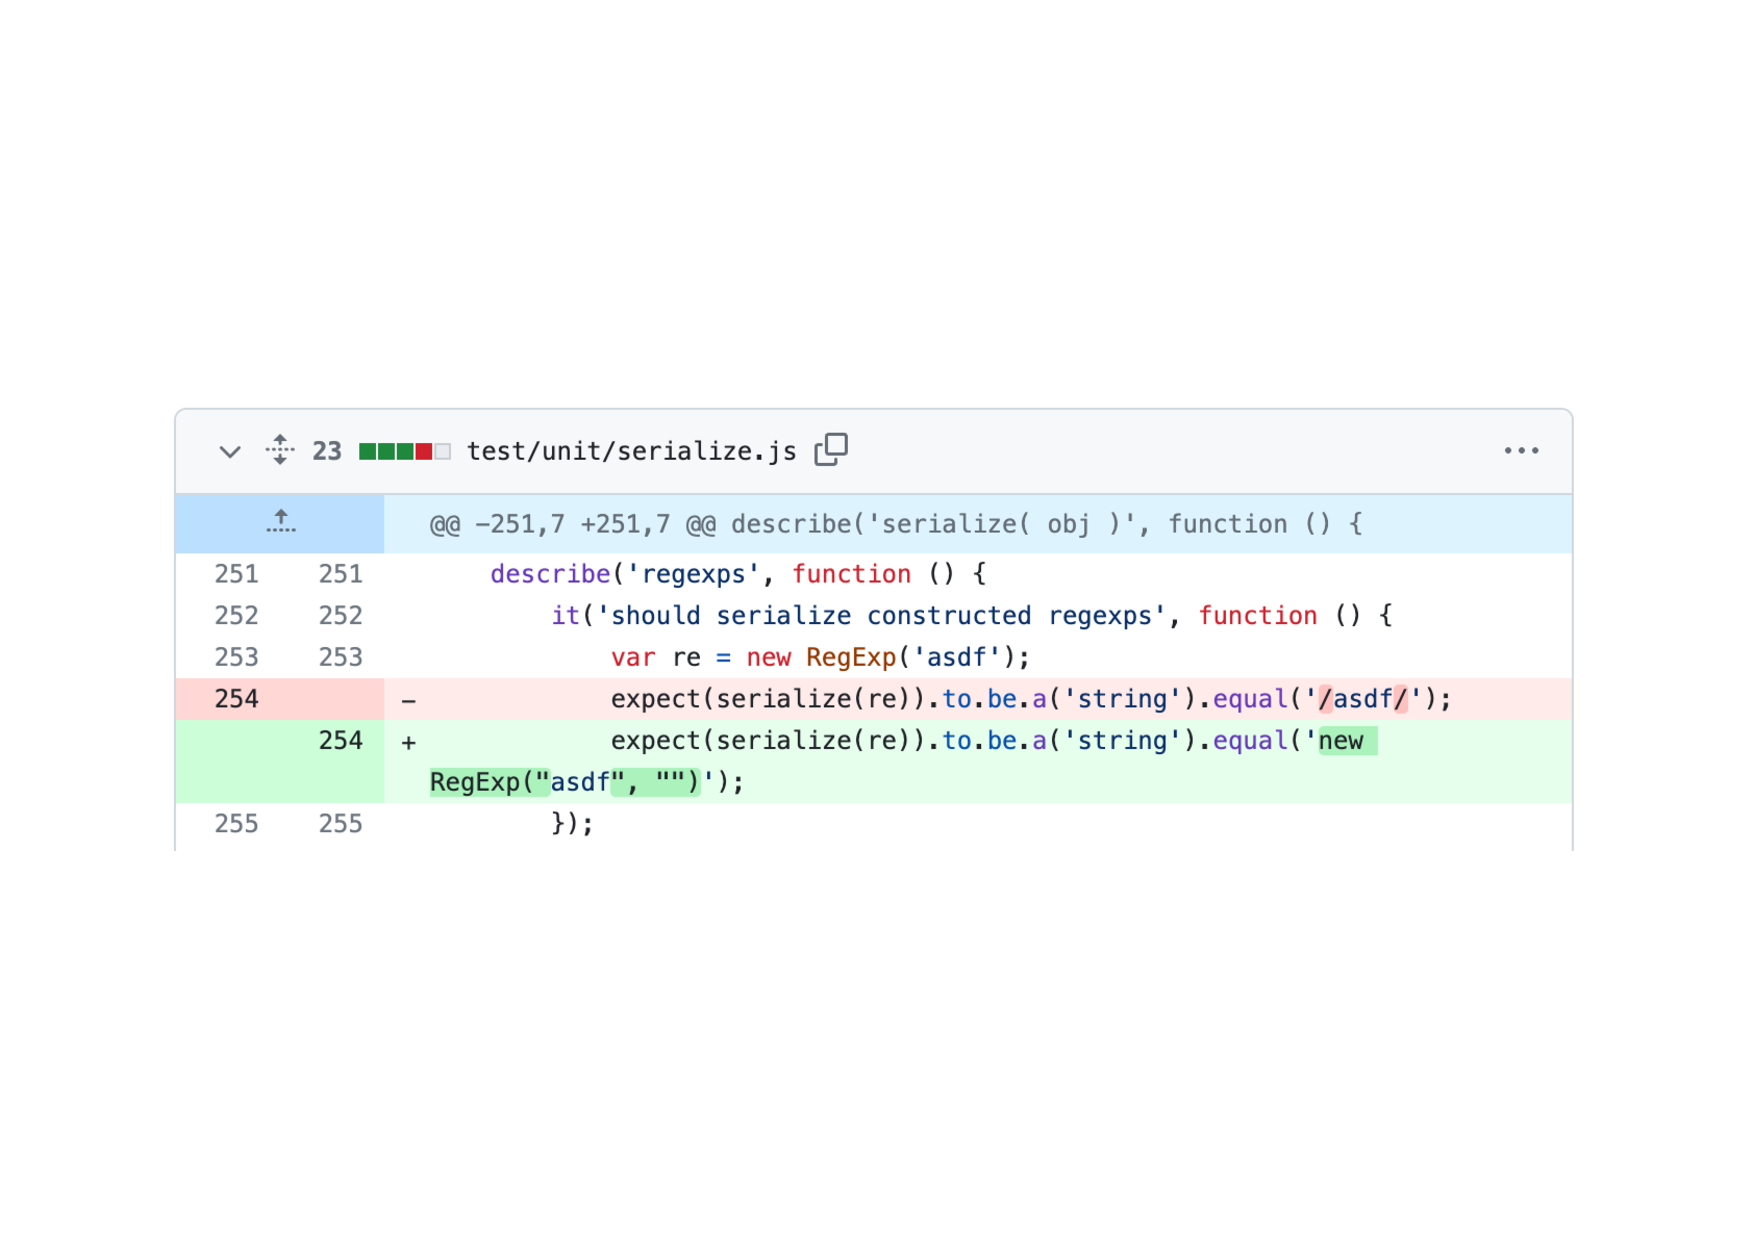
\includegraphics[width=1.0\linewidth]{fig/rq1/serialize-javascript/index.test.pdf}
  \caption{serialize-javascriptのバージョン2.1.0から2.1.1への変更}
\end{figure}


\chapter{RQ1:後方互換性の損失に伴うテストコード変更とは何か?}\label{chap:rq1}

\section{概要}
本章では,ライブラリ更新が後方互換性を含む際,それに伴ってどのようなテストコード変更が行われているかを分析し,後方互換性の損失を検出する手掛かりとなるテストコード変更内容を明らかにする.具体的には,各ライブラリバージョンに対して,後方互換性の有無と,テストコード変更内容を集計する.後方互換性の有無の判定は従来手法と同様,Mujahidらの手法を使用する.各バージョンのテストコードの変更内容は,テストコードの変更差分から目視により分類する.

\section{分析手法}
本分析では,各ライブラリ更新ごとに後方互換性の有無と,テストコード変更内容を目視により集計する.

\subsection{後方互換性の有無の判定}\label{subsec:kouhougokanseinohantei}
後方互換性の有無の判定には,従来手法と同様,Mujahidらの手法を使用する.Mujahidらは,ライブラリの後方互換性の損失をクライアントテストを実行することで検出する手法を提案した\cite{mujahid}.後方互換性を損失する変更を加えられたライブラリバージョンでは,その影響を受けるクライアントテストの結果が更新前後で成功から失敗に変化することを手法の根拠としている.本分析も同様に,対象ライブラリのクライアントに対し,更新後ライブラリを適用し,適用前後でクライアントテストの実行結果が成功から失敗に変わった場合,後方互換性を損失したと判定する.

\subsection{テストコード変更内容の目視分類}
テストコード変更内容を目視分類するために,テストコードの構成要素をまとめる.本研究では,プログラムのテストの中でも単体テストを対象とする.単体テストとは,関数やクラスなどのプログラムを構成する単位(ユニット)が開発者の期待通りに動作するかを検証するテスト手法である.単体テストを実施する際は,テスト対象ユニットに対応するテストスイートを用意する必要がある.テストスイートとは,テストの目的や条件が似ているテストケースの集合を指す.テストケースは,テスト項目の最小単位であり,テスト対象への入力と期待される結果(期待値)の組み合わせで構成する.入力値と期待値を受け取ってプログラムが正しく動作しているか検証する仕組みをアサーションと呼ぶ.

\begin{lstlisting}[caption=Calculator.js, label=Calculator.js]
class Calculator {
  add(a, b) {
    return a + b;
  }
}
\end{lstlisting}

\begin{lstlisting}[caption=Calculator.test.js, label=Calculator.test.js]
import { Calculator } from './Calculator';

describe('Calculator', () => {
  let calculator;

  beforeEach(() => {
    calculator = new Calculator();
  });

  test('should add two positive numbers', () => {
    if (calculator) {
      expect(calculator.add(1, 1)).toBe(2);
    }
  });
});
\end{lstlisting}


Program~\ref{Calculator.js},Program~\ref{Calculator.test.js}は,JavaScriptにおけるテストコードの例を示す.Program~\ref{Calculator.js}は,テスト対象となるクラス{\verb|Calculator|}が定義されている.このクラスに含まれるメソッド{\verb|add()|}は,2つの引数を受け取り足し合わせた値を返す.Program~\ref{Calculator.test.js}は,{\verb|Calculator|}クラスを単体テストによって検証するファイルで,JavaScript向けテストフレームワークJest\footnote{\url{https://jestjs.io/}}を使用して記述している.

Program~\ref{Calculator.test.js}は,3行目の{\verb|describe|}関数でテストスイートを宣言し,10行目の{\verb|test|}関数により1つのテストケースを定義している.テストスイートやテストケースは,何を検証するかが記述されるラベルと,動作を検証するテスト用関数を引数に取る.6行目から7行目の{\verb|beforeEach|}関数で,テストフィクスチャと呼ばれる,テストデータの初期化などのテストの事前条件を定義する.例では,{\verb|Calculator|}クラスをインスタンス化している.10行目から12行目で定義されるテストケースは,11行目で{\verb|if|}文によりテストの前提条件を記述し,12行目のアサーションで{\verb|Calculator.add()|}に対し{\verb|1|}と{\verb|1|}を入力したときの動作を検証している.この場合,期待する結果は{\verb|2|}であるため,{\verb|toBe|}節で結果が{\verb|2|}となる.

以上を踏まえ,本論文では,テストコードの変更内容として11件の内容を考慮する.

\begin{itemize}
  \setlength{\itemsep}{0cm}
  \item テストスイートの追加
  \item テストスイートの削除
  \item テストケースの追加
  \item テストケースの削除
  \item アサーションの追加
  \item アサーションの削除
  \item アサーションの入力値の変更
  \item アサーションの期待値の変更
  \item テストの前提条件の変更
  \item テストフィクスチャの変更
  \item リファクタリング
\end{itemize}

リファクタリングは,テストスイート・テストケースのラベルの変更,テストフレームワークの変更,可読性向上のためのフォーマッティングなどテストコードの振る舞いに関わらない変更を含む.

\section{データセット}\label{rq1:datasets}
データセットとして,従来研究\cite{matsuda}で収集されたライブラリバージョン群を使用する.従来研究では,ライブラリの人気度を示すnpmスコア~\footnote{\url{https://npms.io}}が上位500件以内で,各バージョンのコミットにおけるテスト実行時の成功率が100%であることを条件にnpm\footnote{\url{https://www.npmjs.com/}}から2,111件のライブラリバージョンを収集した.本調査では,このデータセットから,ライブラリテストに変更があるライブラリバージョン1,027件を抽出し,95%の信頼区間でサンプリングした280件を対象とする.分析対象とするライブラリと,各ライブラリのいずれかに依存するクライアントとの組み合わせは,Mujahidらのデータセットから抽出した.

\section{分析結果}\label{seq:rq1-result}

\begin{figure}[t]
  \centering
  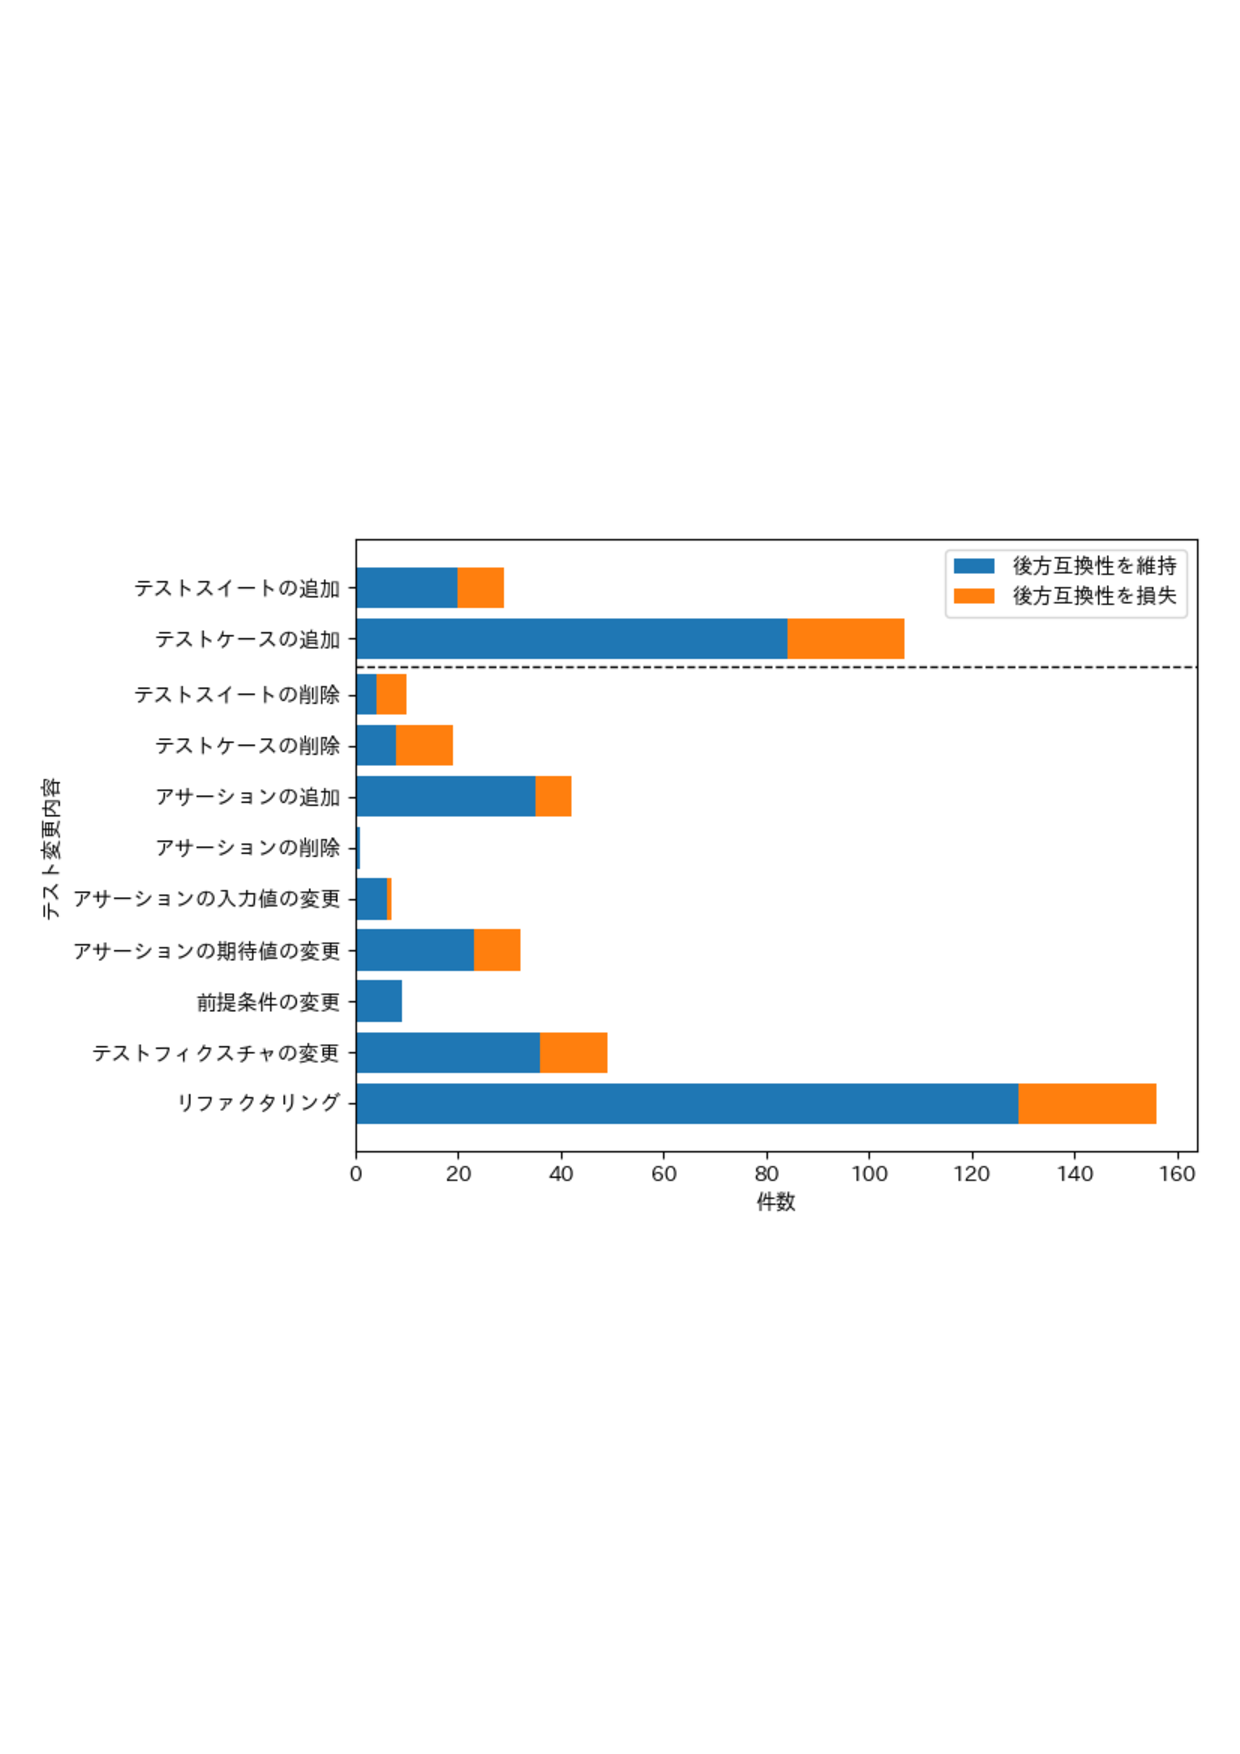
\includegraphics[width=1.0\linewidth]{fig/barh-test-pattern.pdf}
  \caption{テスト変更内容ごとの実際の後方互換性}
  \label{fig:test_pattern}
\end{figure}

図\ref{fig:test_pattern}は,テスト変更内容ごとの後方互換性の有無を横棒積み上げ棒グラフで示す.縦軸は各テストコード変更内容,横軸は
各テストコード変更の発生件数である.リファクタリングは件数も多くほとんどが後方互換性を維持しているため,後方互換性の損失に伴うテストコード変更内容とは言えず,従来手法で誤検出となる大きな原因であるとわかる.テストスイートの追加,テストケースの追加,アサーションの追加は,後方互換性を維持するライブラリ更新に伴う割合が後方互換性を損失するライブラリ更新に伴う割合より高い.これらの変更は従来手法でテスト追加に分類され後方互換性を維持すると判定されるため,主な誤検出の原因ではないとわかる.ただし,後方互換性を損失するライブラリ更新に伴ってテストコードが追加される場合もある.具体的な例は\ref{subsec:add-test}章で述べる.テストスイートの削除,テストケースの削除は,後方互換性を損失するライブラリ更新に伴う割合が後方互換性を維持するライブラリ更新に伴う割合より高い.これらの変更は従来手法でテスト削除に分類され後方互換性を損失すると判定されるため,主な誤検出の原因ではないとわかる.ただし,後方互換性を維持するライブラリ更新に伴ってテストコードが削除される場合もある.具体的な例は\ref{subsec:delete-test}章で示す.アサーションの入力値の変更,アサーションの期待値の変更,前提条件の変更は後方互換性を維持するライブラリ更新に伴う割合が後方互換性を損失するライブラリ更新に伴う割合より高い.これらの変更は従来手法でテスト変更に分類され後方互換性を損失すると判定されるため,誤検出の原因であるとわかる.ただし,後方互換性の損失に伴って,アサーションの入力値,期待値が変更される場合もある.具体的な例は,\ref{subsec:change-test}章で示す.テストフィクスチャの変更は,テストデータの初期化や事前条件を定義する性質上,変更時のテストコードの影響範囲が広く,後方互換性の損失との関係を分析することが困難であるため,本研究では対象としない.

\section{考察}
\ref{seq:rq1-result}章の結果をもとに,後方互換性の損失を検出する手掛かりとなるテストコード変更内容について例を挙げながら考察する.

\subsection{テストコード追加}\label{subsec:add-test}

テストコード追加は,従来手法で後方互換性を維持すると判定されるが,ライブラリの後方互換性の損失に伴ってテストコードが追加される場合がある.例として,JavaScriptオブジェクトを文字列に変換するAPIを提供するライブラリserialize-javascriptのバージョン1.6.1から1.7.0へのマイナーアップデート\footnote{\url{https://github.com/yahoo/serialize- javascript/compare/v1.6.1...v1.7.0}}を挙げる.図\ref{fig:rq1.insert-test-src}はソースコードの変更差分,図\ref{fig:rq1.insert-test-test}はテストコードの変更差分を示す.この変更では,関数{\verb|serialize|}に,JavaScriptの{\verb|Map|}型のデータを文字列に変換する機能が追加された(図\ref{fig:rq1.insert-test-src},155行目から157行目).この変更に伴って,関数{\verb|serialize|}に関するテストスイート(図\ref{fig:rq1.insert-test-test},7行目)に,新しく{\verb|Map|}型のデータが正確に文字列に変換されるかを検証するテストスイートが追加された(図\ref{fig:rq1.insert-test-test},201行目から220行目).バージョン1.6.1では,関数{\verb|serialize|}は{\verb|Map|}型の入力を文字列に変換する機能を持っていないため,文字列に変換されないことに依存しているクライアントはバージョン更新の際に返り値が新しくなったことによる影響を受ける.このようなAPIの機能拡張による後方互換性の損失は,図\ref{fig:rq1.insert-test-test}で示すように既存のテストスイート内にテストコードが追加されるという特徴があるため,既存のテストスイート内にテストスイート,テストケース,アサーションが追加された場合,ライブラリの後方互換性が損失したと判断できると考えられる.

\begin{figure}[t]
  \centering
  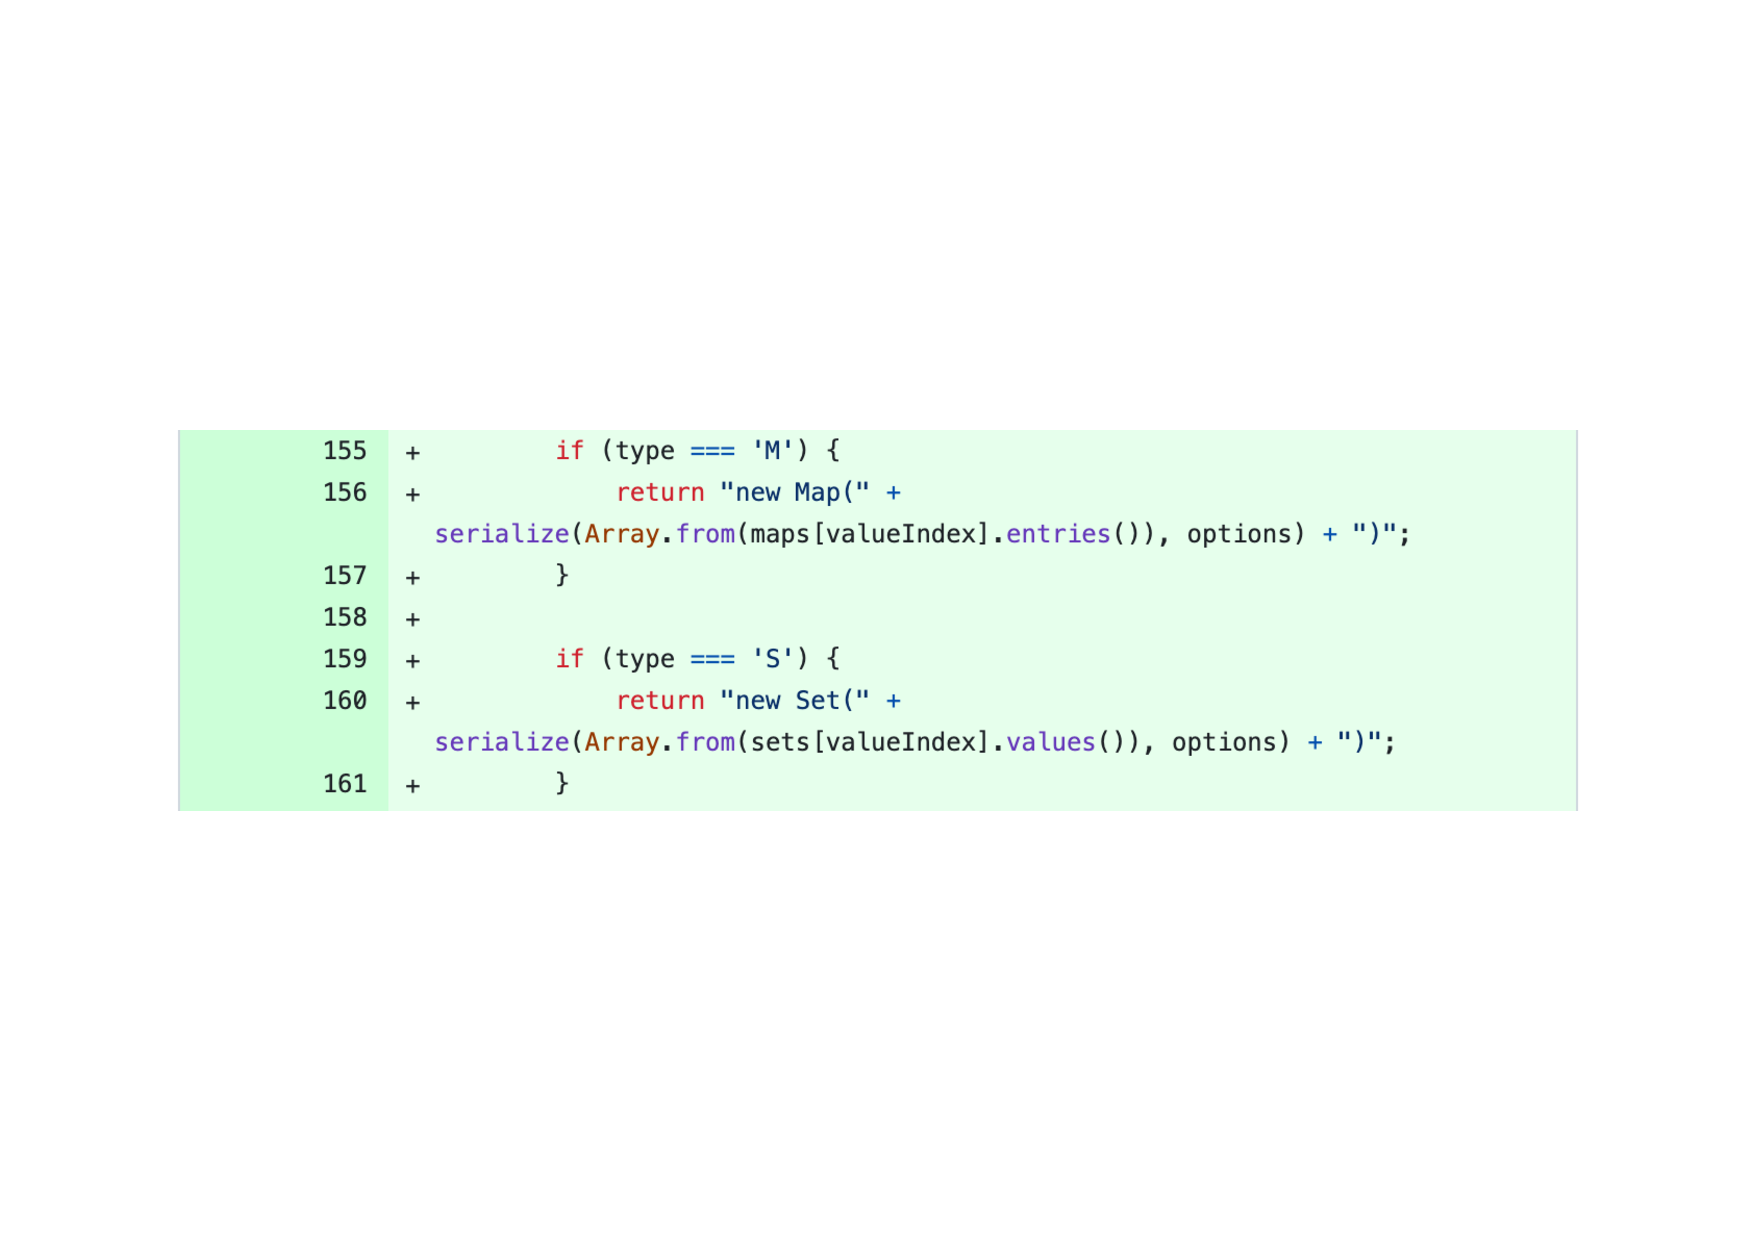
\includegraphics[width=1.0\linewidth]{fig/rq1/set-map/map.pdf}
  \caption{serialize-javascriptのバージョン1.6.1から1.7.0のソースコード変更差分}
  \label{fig:rq1.insert-test-src}
\end{figure}

\begin{figure}[t]
  \centering
  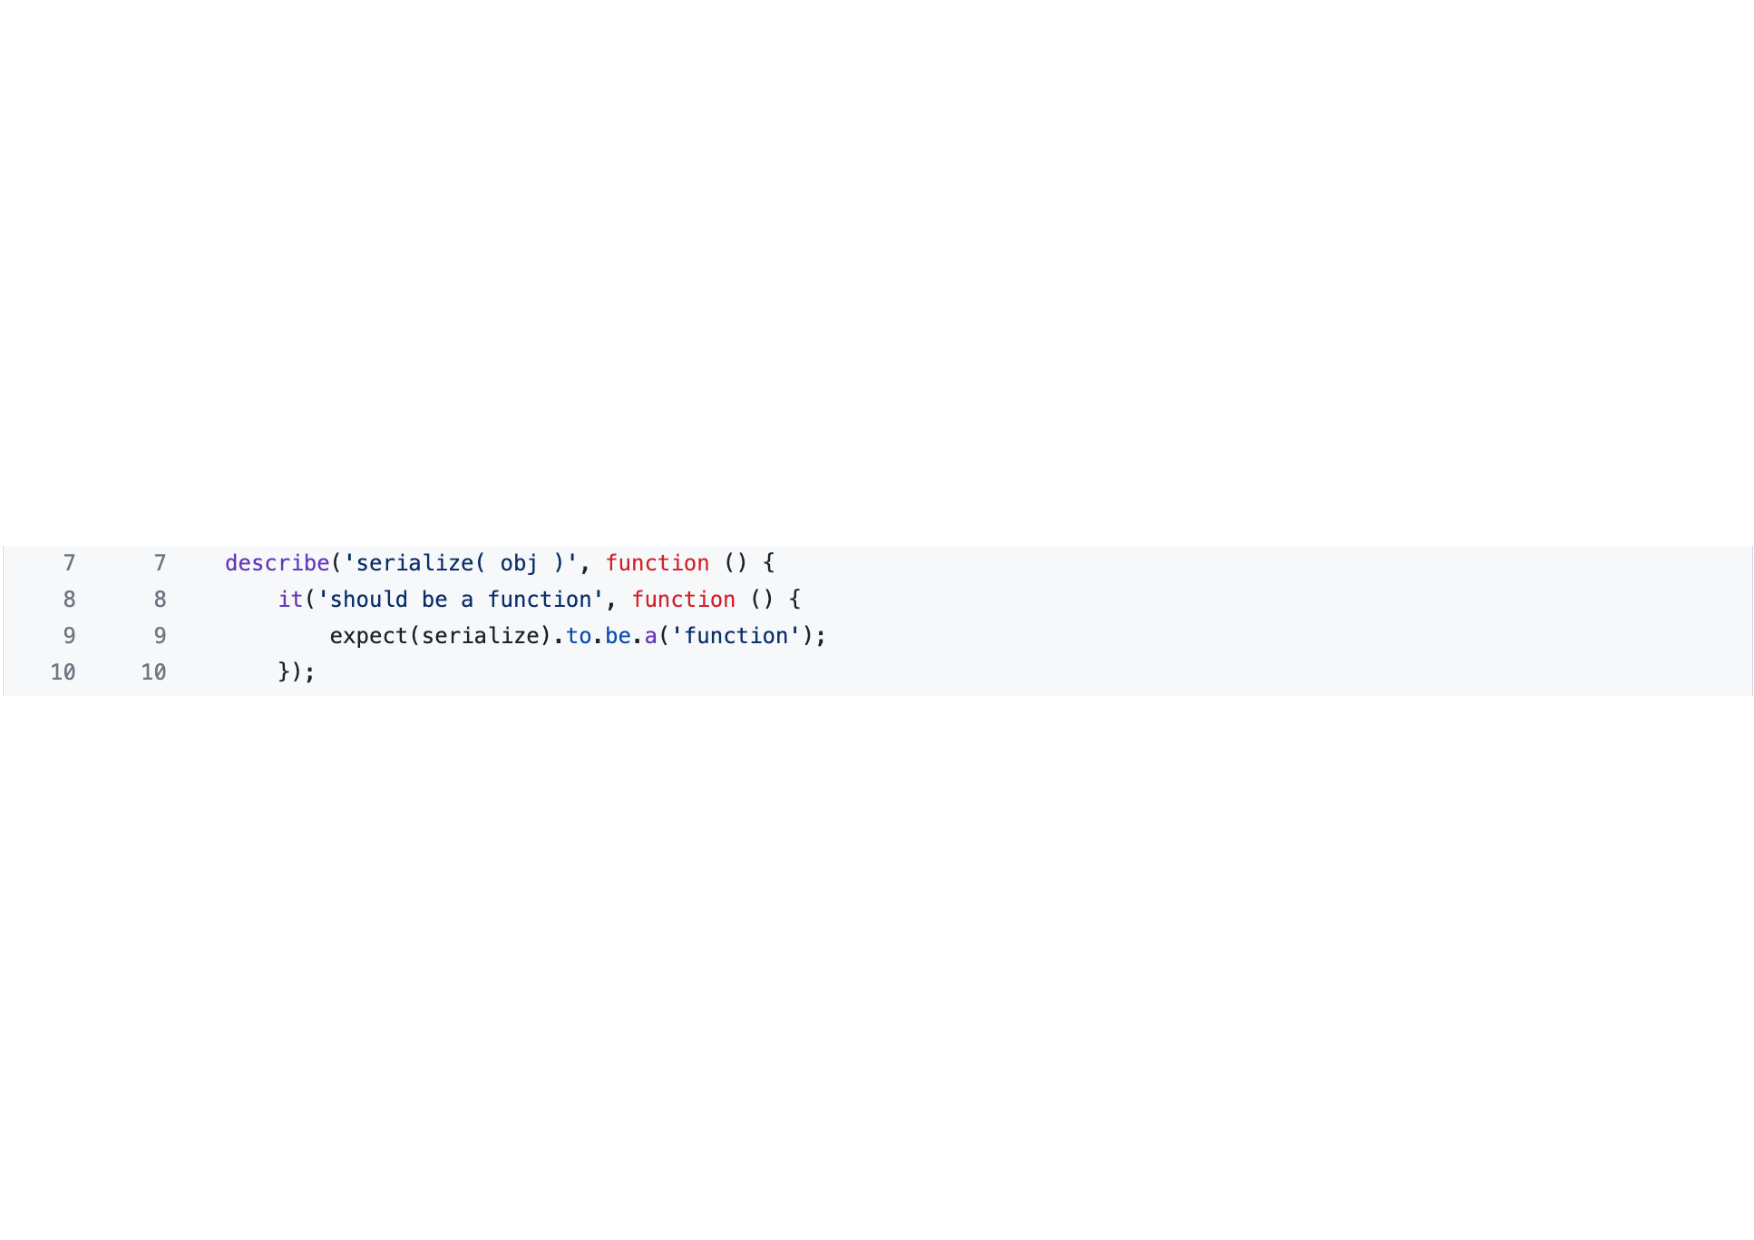
\includegraphics[width=1.0\linewidth]{fig/rq1/set-map/map.test.1.pdf}
  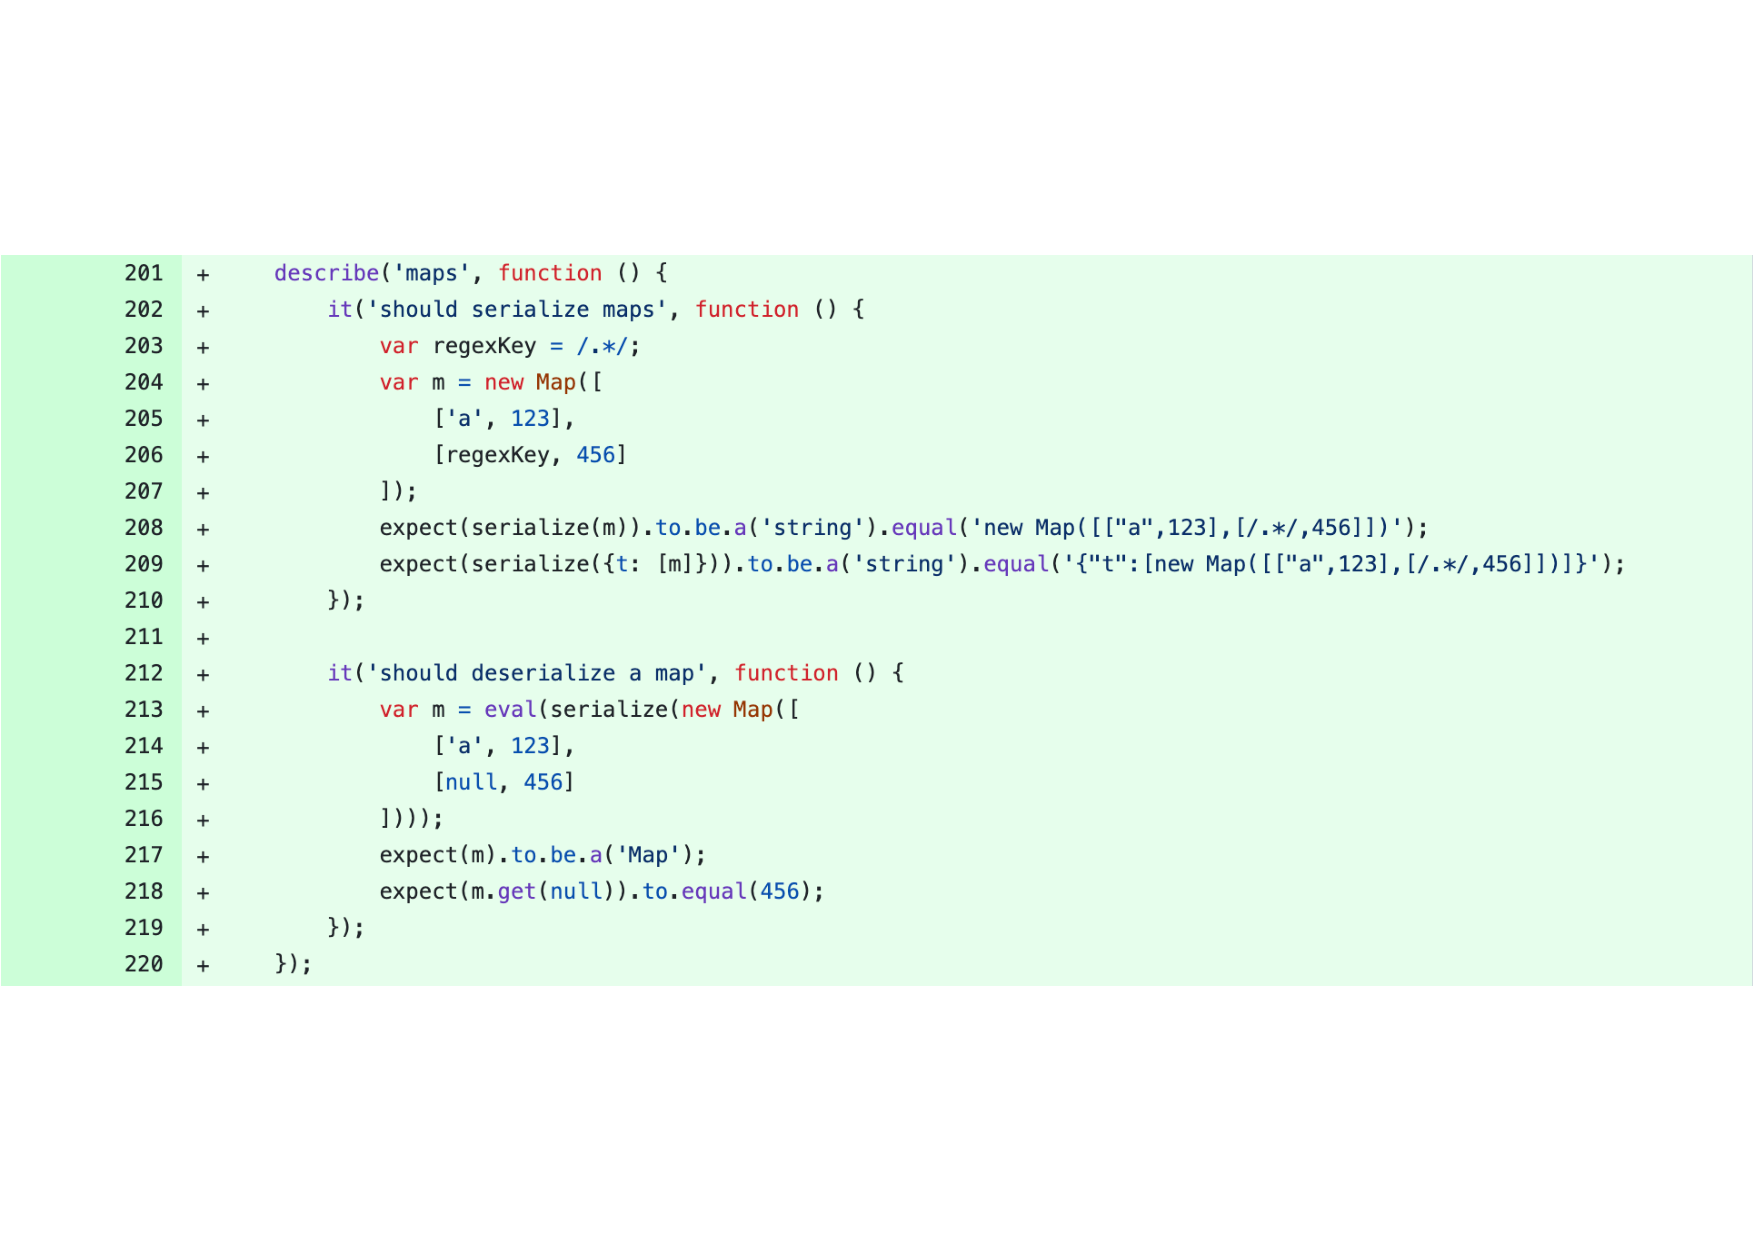
\includegraphics[width=1.0\linewidth]{fig/rq1/set-map/map.test.2.pdf}
  \caption{serialize-javascriptのバージョン1.6.1から1.7.0のテストコード変更差分}
  \label{fig:rq1.insert-test-test}
\end{figure}

\subsection{テストコード削除}\label{subsec:delete-test}

\begin{figure}[t]
  \centering
  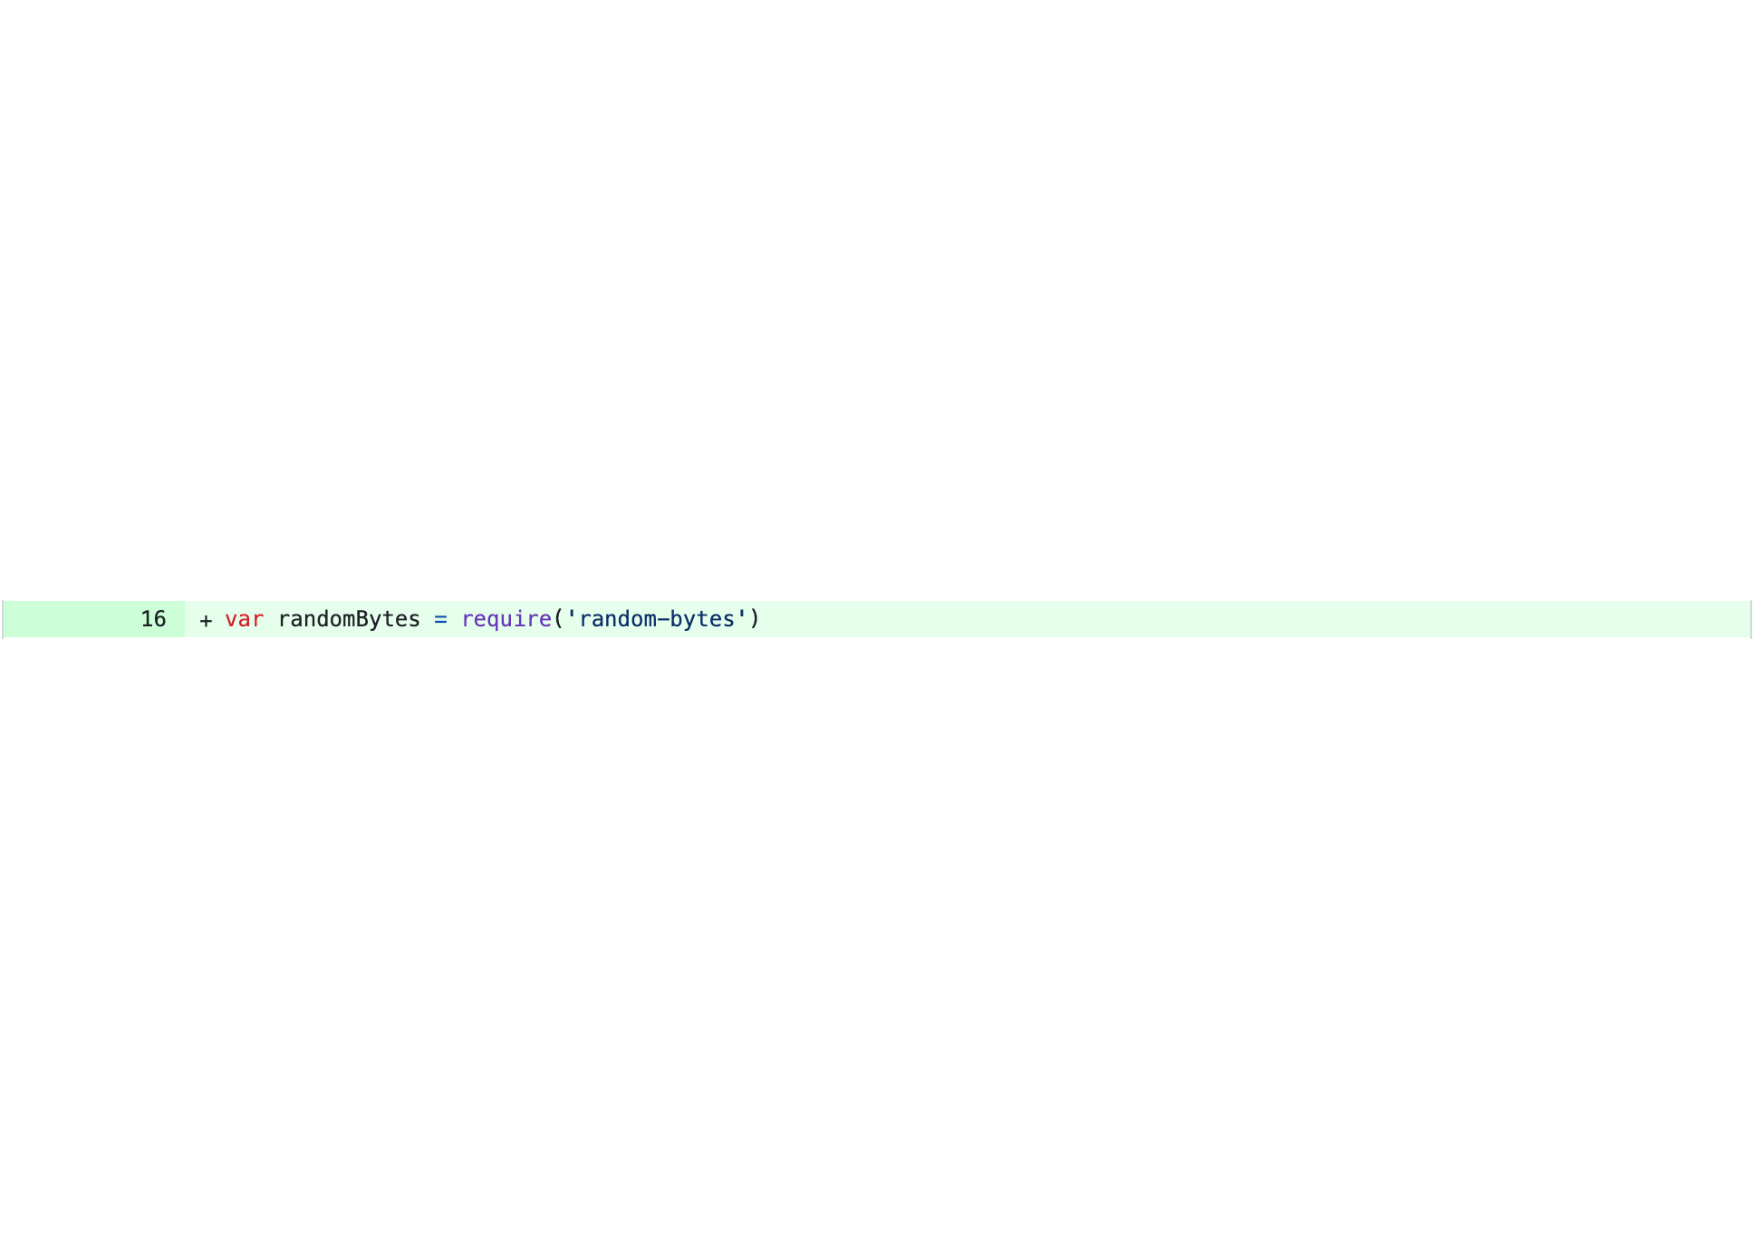
\includegraphics[width=1.0\linewidth]{fig/rq1/uuid/randomBytes2.pdf}
  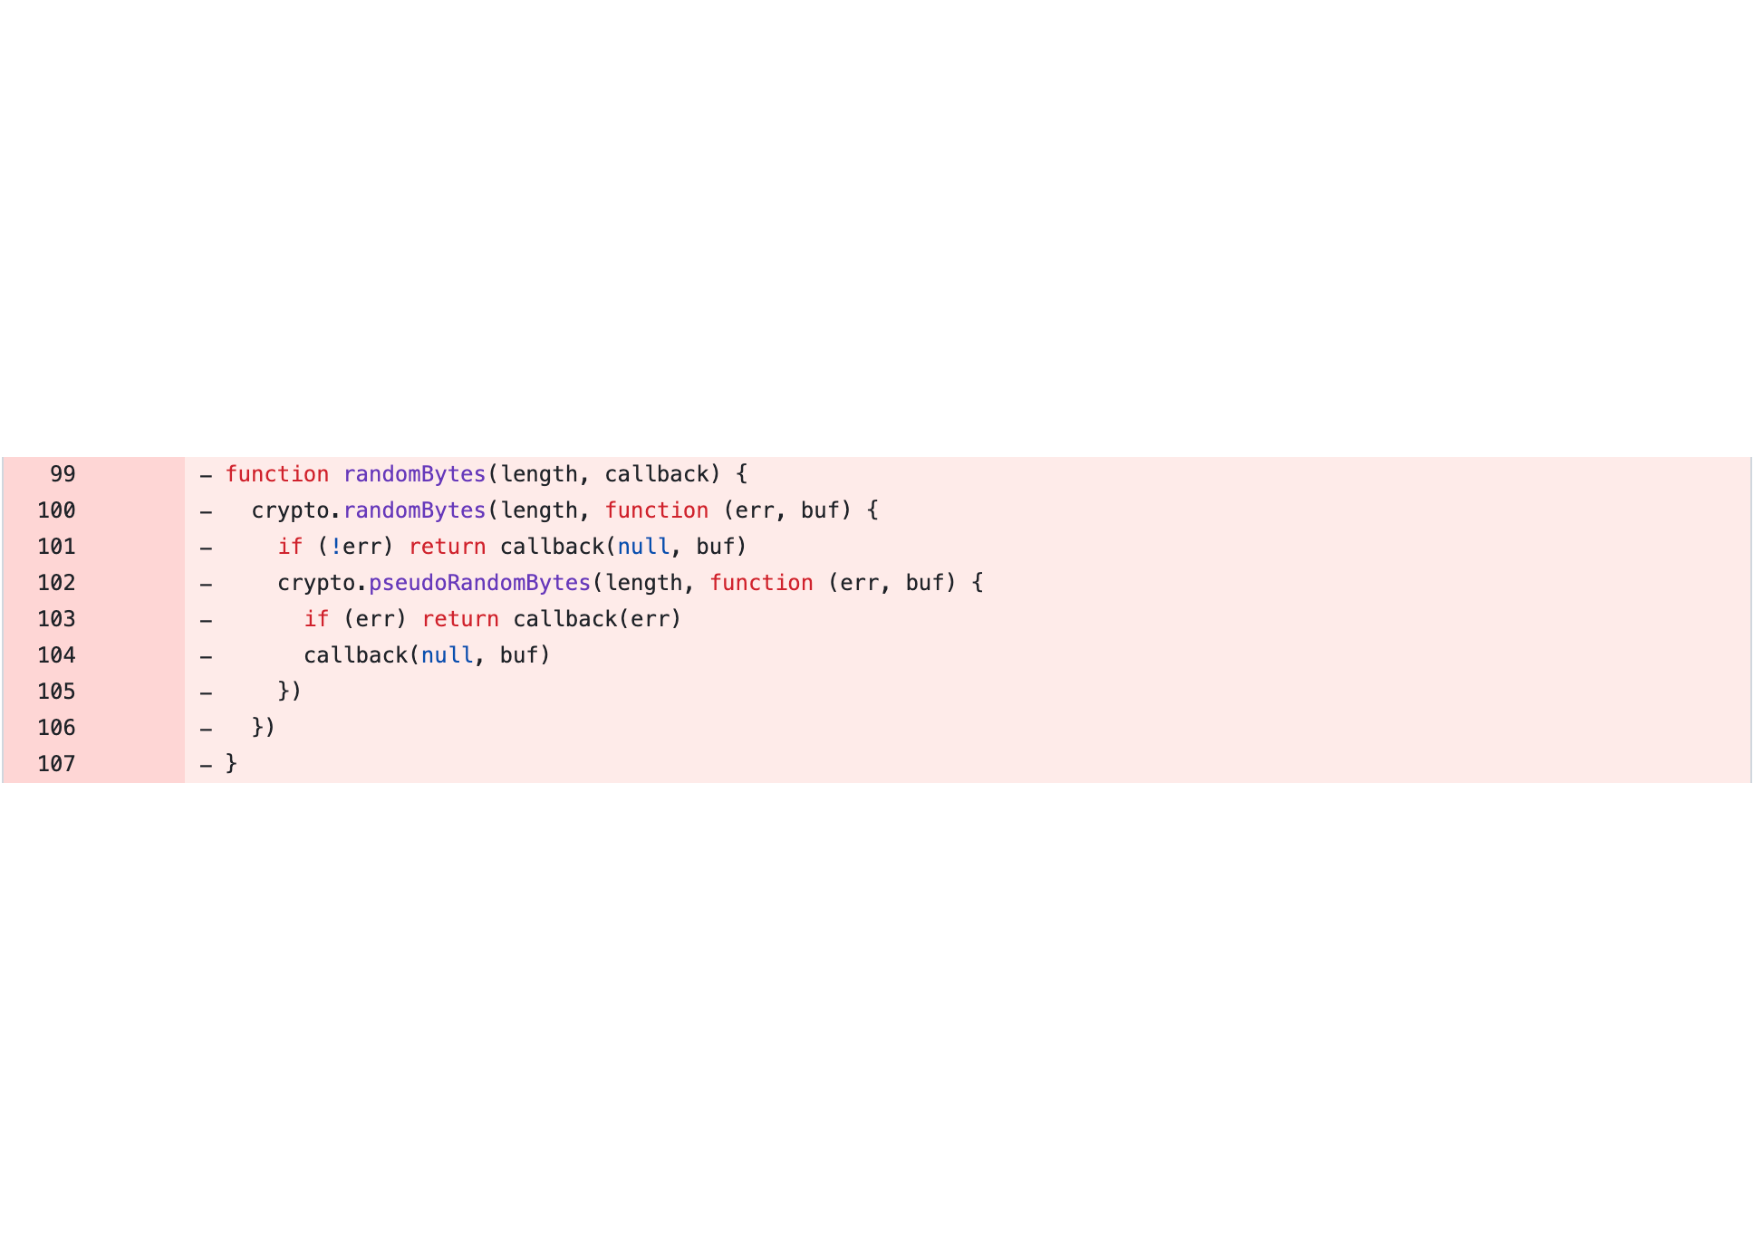
\includegraphics[width=1.0\linewidth]{fig/rq1/uuid/randomByte.pdf}
  \caption{uid-safeのバージョン2.0.0から2.1.0のソースコード変更差分}
  \label{fig:rq1.delete-test-src}
\end{figure}

\begin{figure}[t]
  \centering
  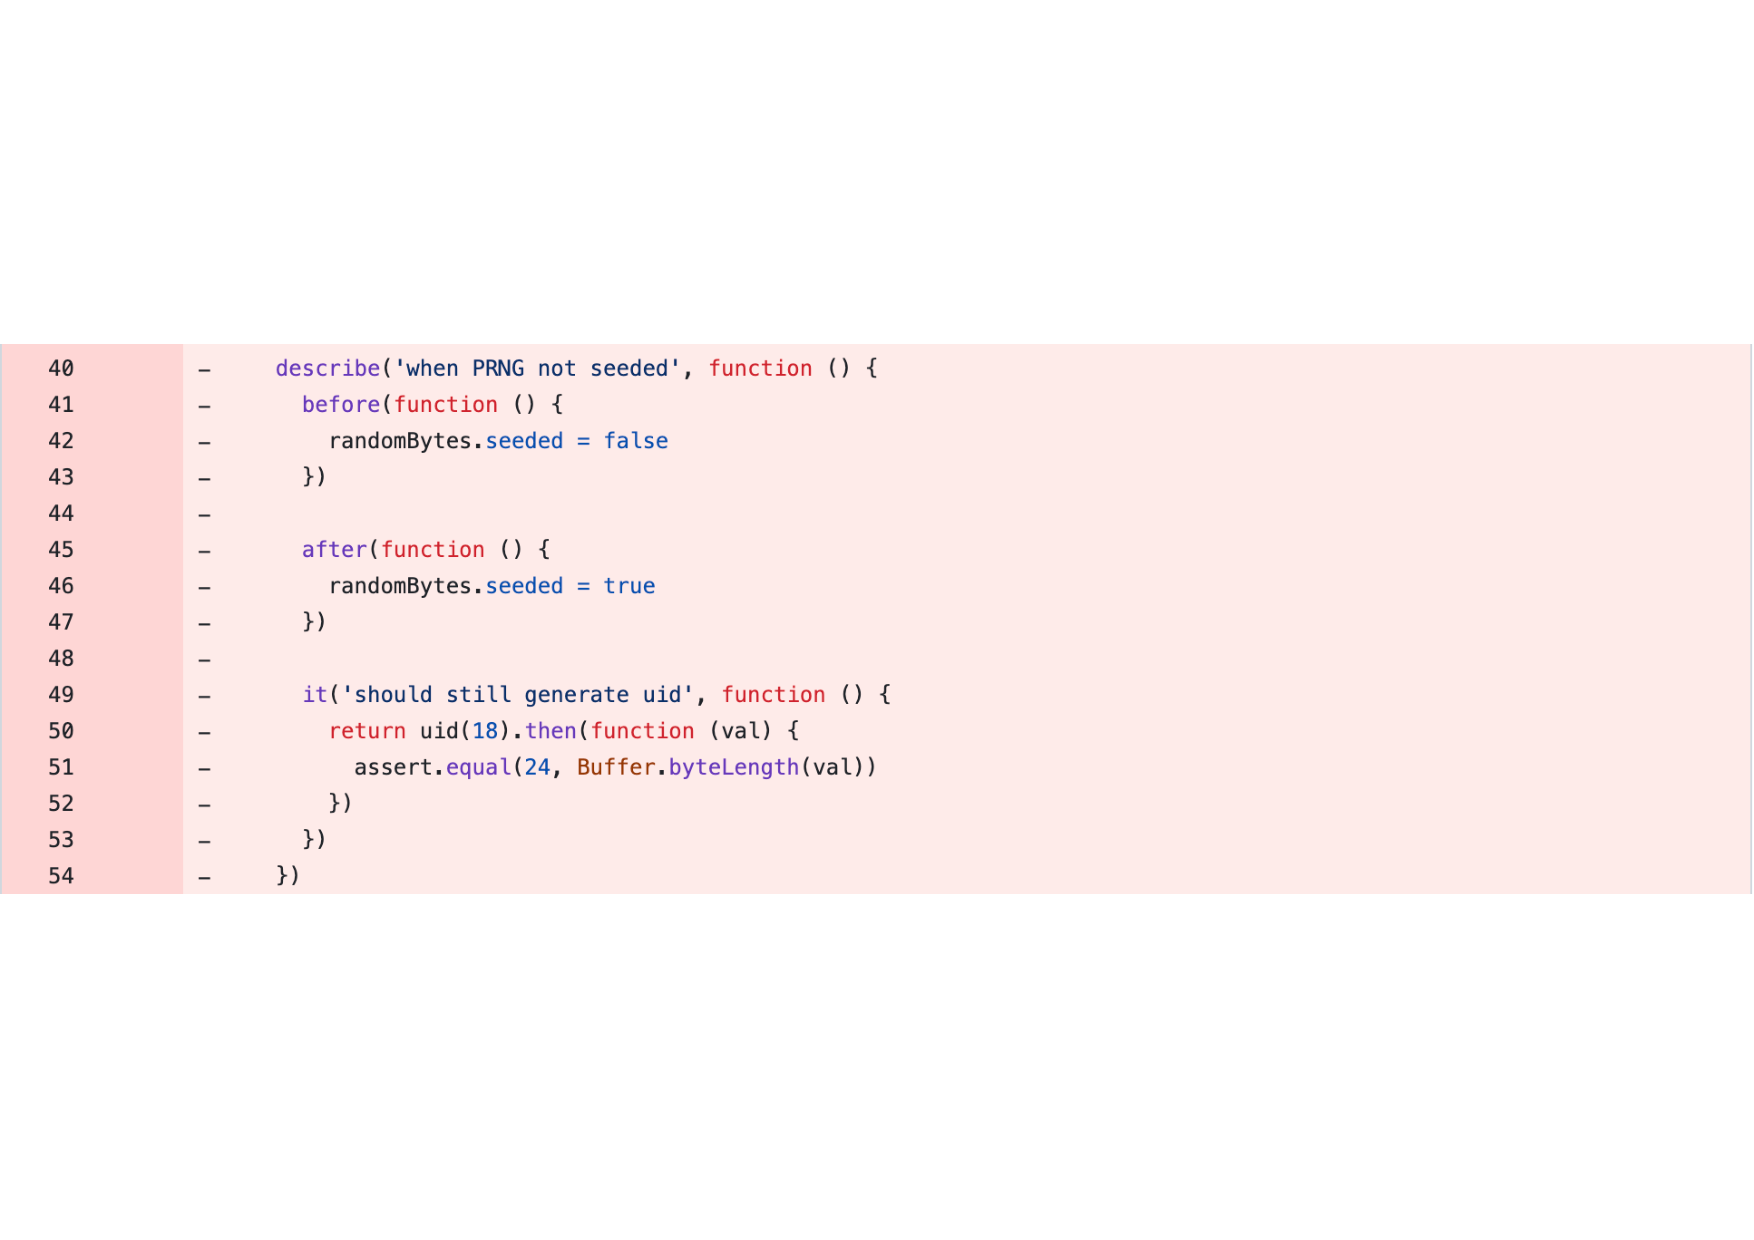
\includegraphics[width=1.0\linewidth]{fig/rq1/uuid/randomByte-test.pdf}
  \caption{uid-safeのバージョン2.0.0から2.1.0のテストコード変更差分}
  \label{fig:rq1.delete-test-test}
\end{figure}

テストコード削除は,従来手法で後方互換性を損失すると判定される.ライブラリが提供するAPIを削除することによる後方互換性の損失は,対象となるAPIのテストコードを同時に削除することが考えられるため,テストスイート,テストケースが削除された場合,ライブラリの後方互換性が損失したと判断できる.一方で,ライブラリは後方互換性を維持しているが,テストコードが削除される場合がある.例として,暗号化されたUIDを生成するAPIを提供するライブラリuid-safeのバージョン2.0.0から2.1.0へのマイナーアップデート\footnote{\url{https://github.com/crypto-utils/uid-safe/compare/2.0.0...2.1.0}}を挙げる.図\ref{fig:rq1.delete-test-src}はソースコードの変更差分,図\ref{fig:rq1.delete-test-test}はテストコードの変更差分を示す.この変更では,セキュリティ上の問題から,ランダムなバイト列を生成する関数{\verb|randomBytes|}を削除(図\ref{fig:rq1.delete-test-src},99行目から107行目)し,同等のモジュールに置き換えている(図\ref{fig:rq1.delete-test-src},16行目).この変更に伴って,関数{\verb|randomBytes|}の動作を検証するテストスイートが削除されている(図\ref{fig:rq1.delete-test-test},40行目から54行目).モジュールの置き換え前後で関数{\verb|randomBytes|}の振る舞いが全く同じ場合,後方互換性が維持される.本研究では,\ref{subsec:kouhougokanseinohantei}章で述べた通り,後方互換性の有無の判定にクライアントテストを利用している.このようなモジュールに置き換える例では,振る舞いの変化が限定的になるため,クライアントテストが捉えられず後方互換性を維持したと誤判定されることが考えられる.誤判定を防ぐには実際に影響を受けるクライアントの特定が必要になるが本研究では今後の課題とする.

\subsection{アサーションの入力値,期待値の変更}\label{subsec:change-test}

\begin{figure}[t]
  \centering
  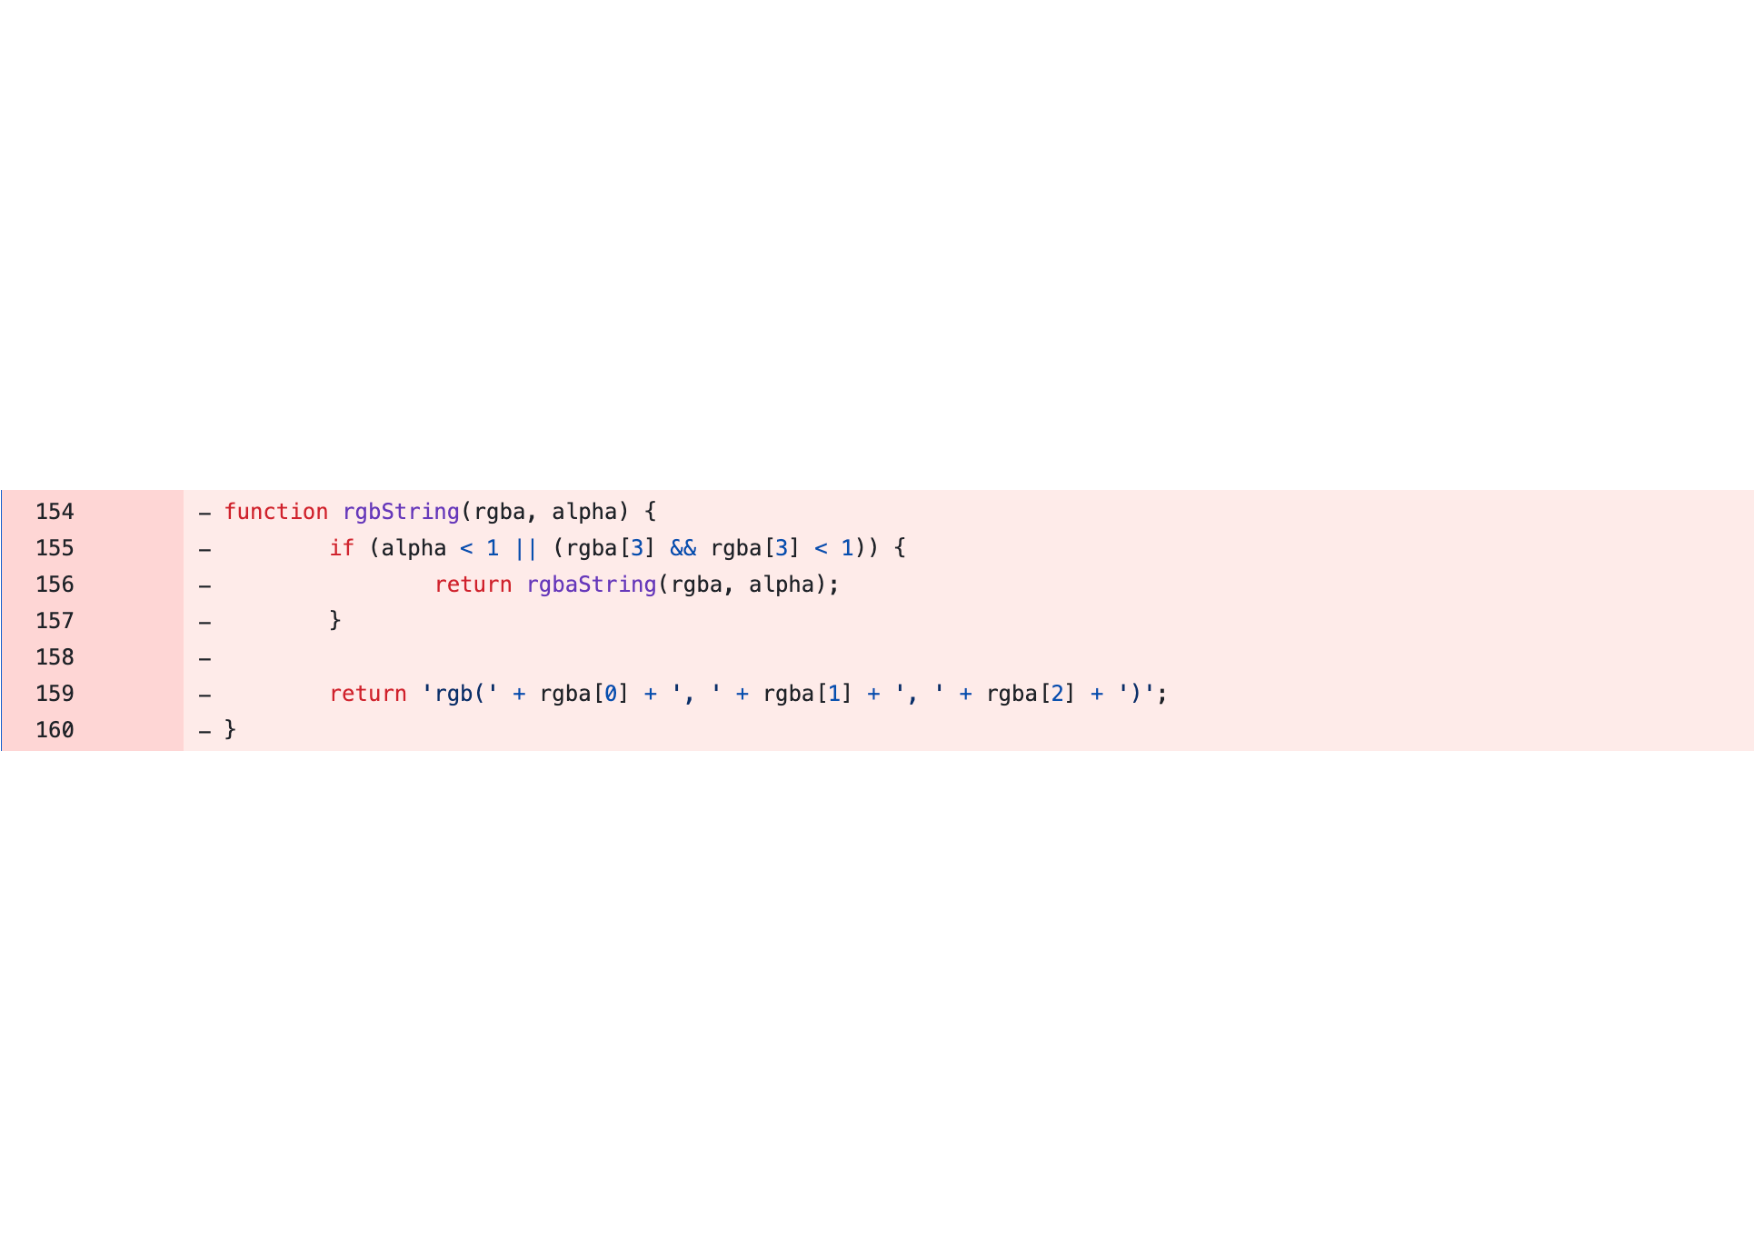
\includegraphics[width=1.0\linewidth]{fig/rq1/rgb/rgb-src.pdf}
  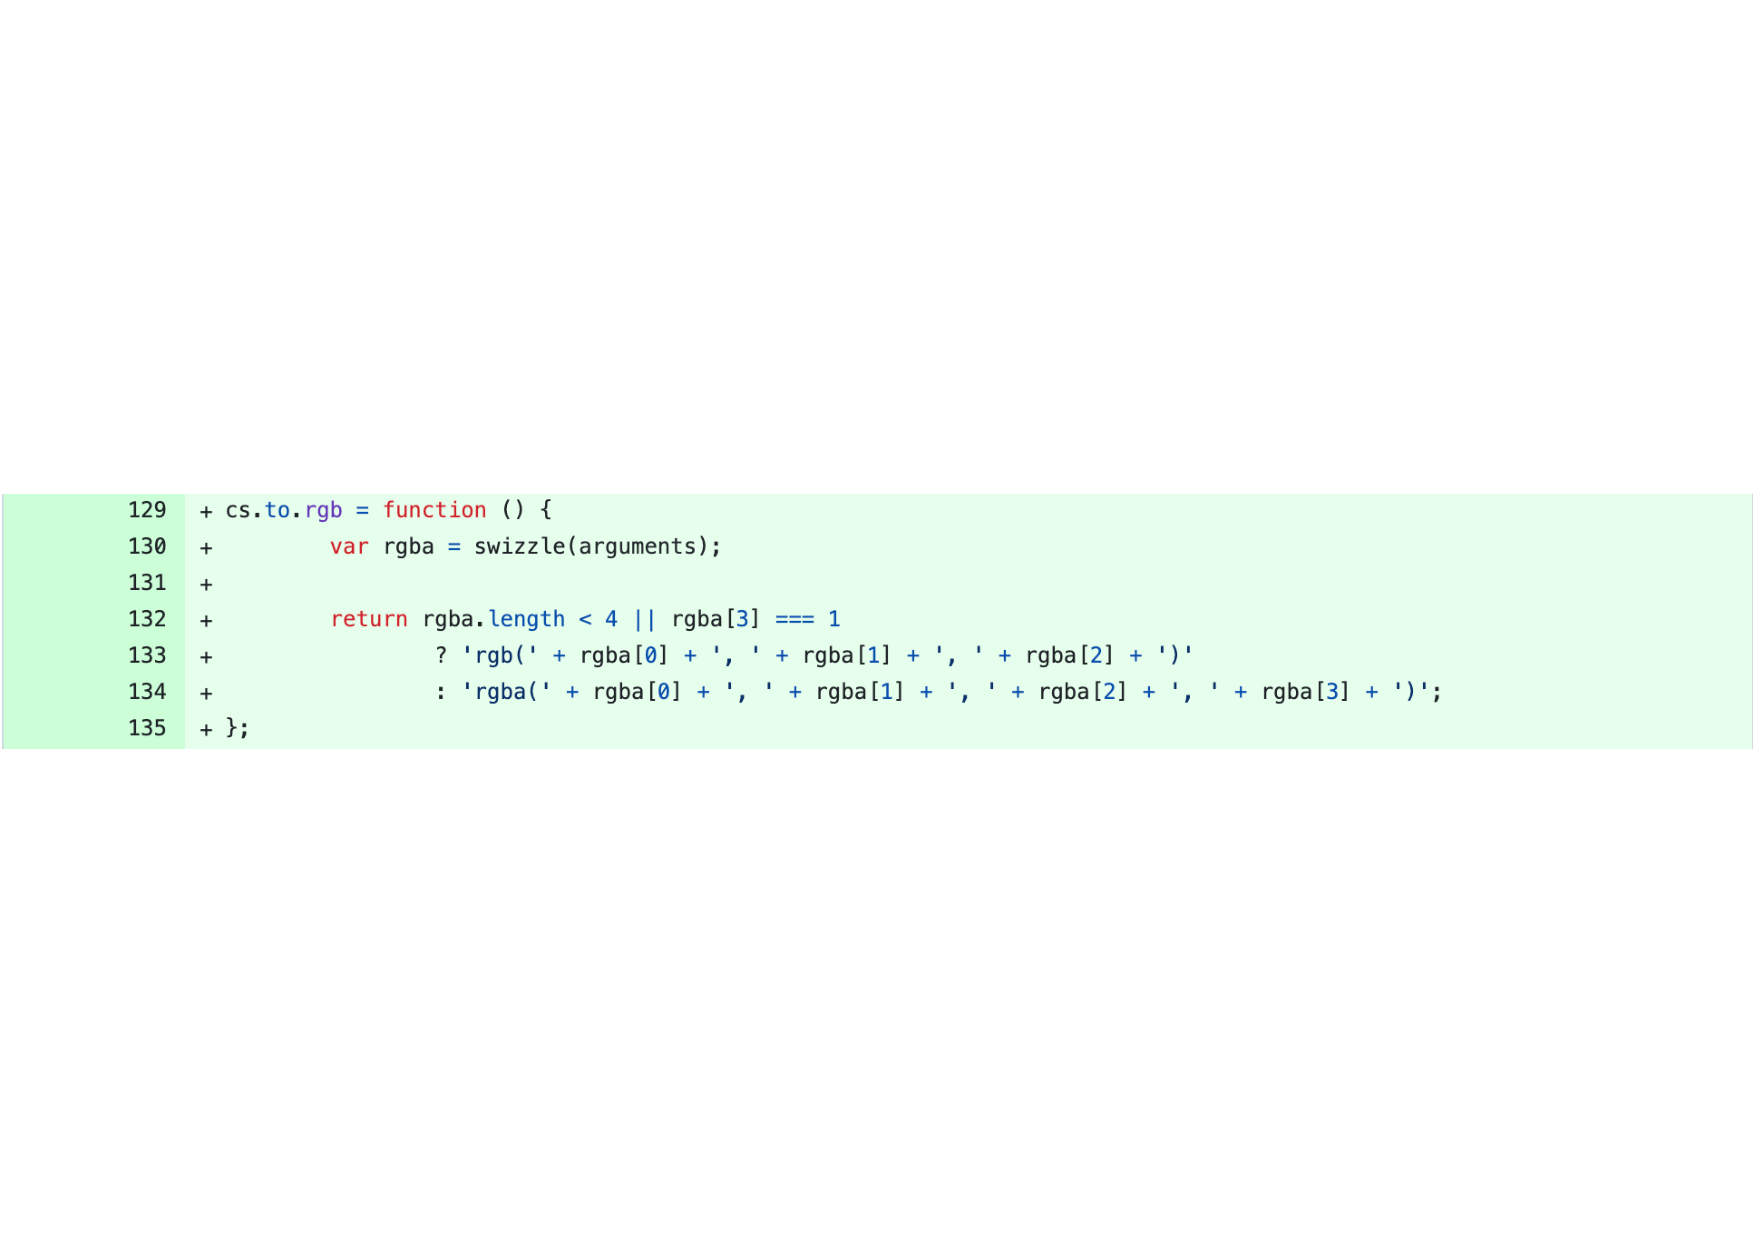
\includegraphics[width=1.0\linewidth]{fig/rq1/rgb/rgb-src-1.pdf}
  \caption{color-stringのバージョン0.4.0から1.0.0のソースコード変更差分}
  \label{fig:rq1.change-test-input-src}
\end{figure}

\begin{figure}[t]
  \centering
  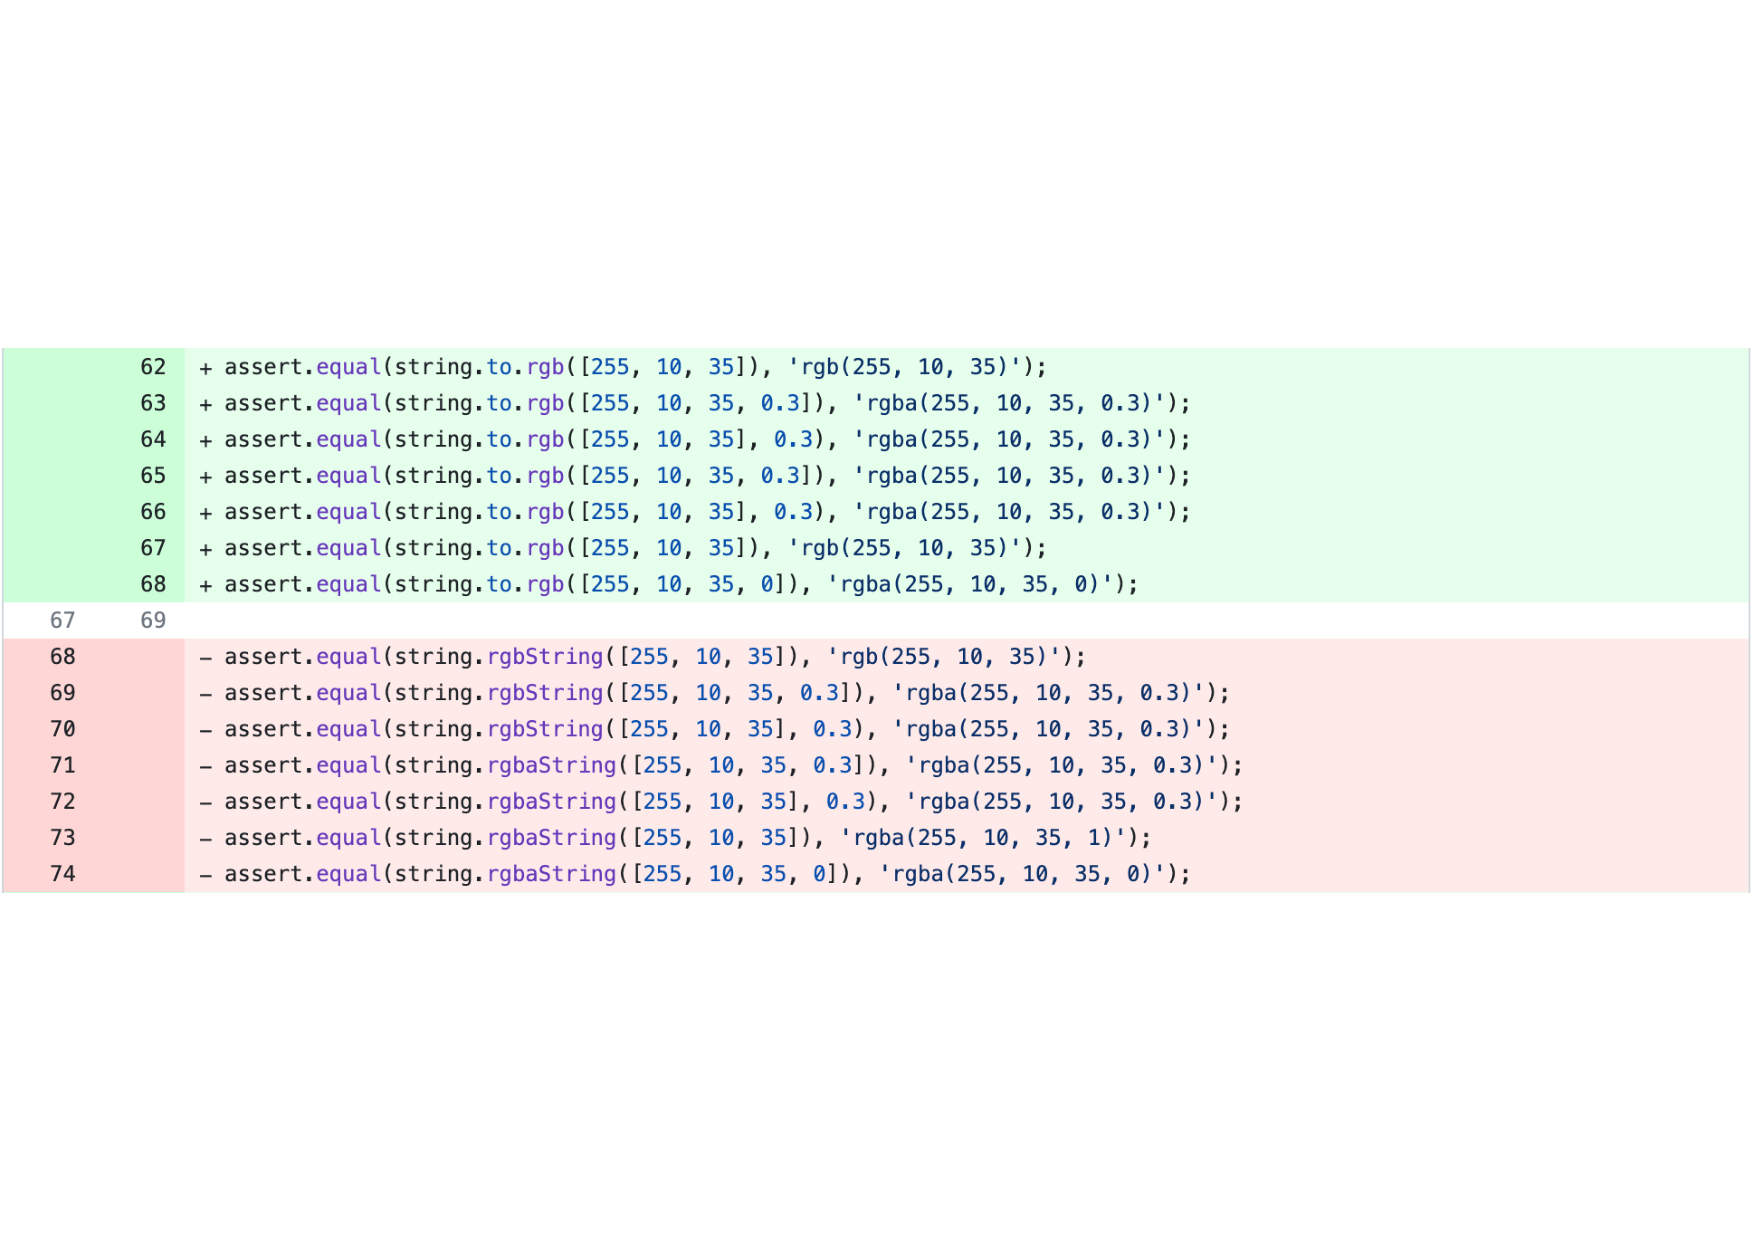
\includegraphics[width=1.0\linewidth]{fig/rq1/rgb/rgb-test.pdf}
  \caption{color-stringのバージョン0.4.0から1.0.0のテストコード変更差分}
  \label{fig:rq1.change-test-input-test}
\end{figure}

\begin{figure}[t]
  \centering
  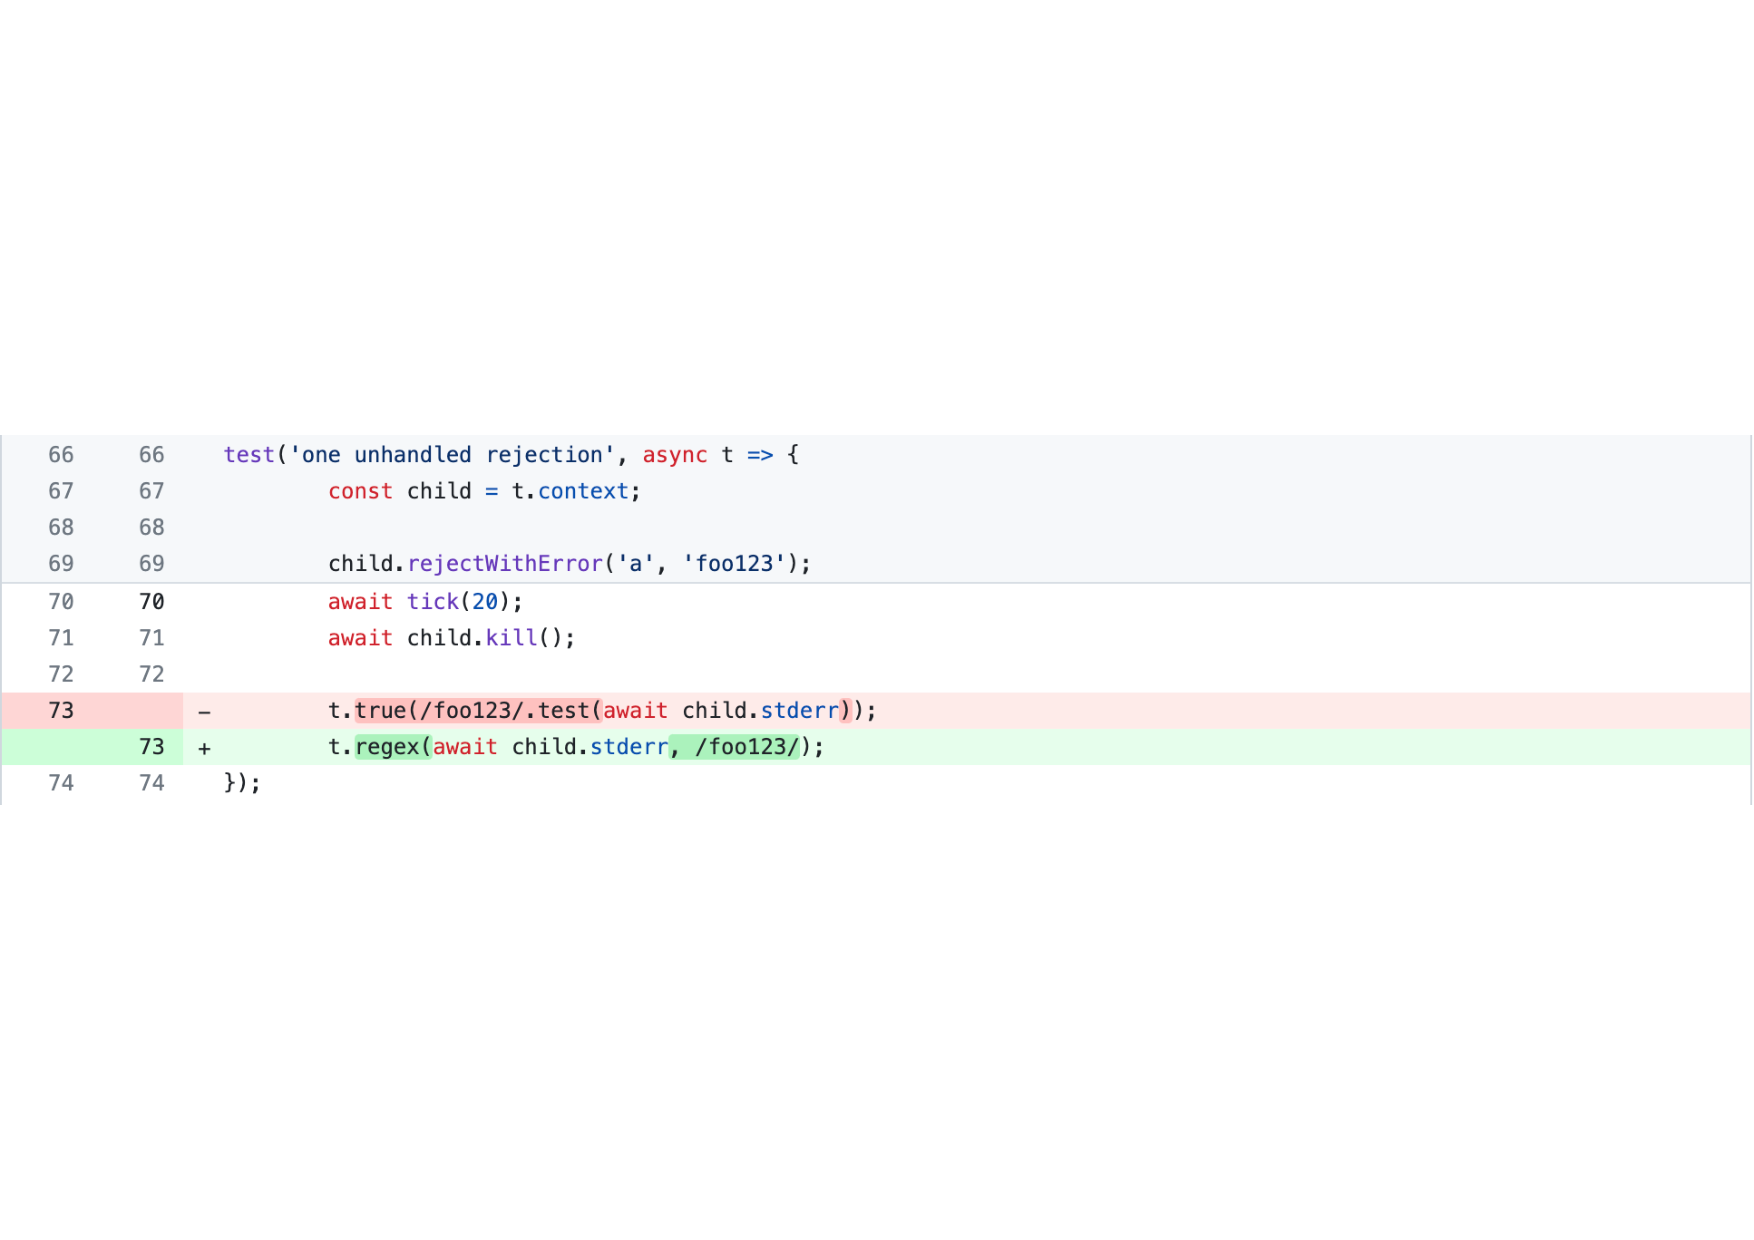
\includegraphics[width=1.0\linewidth]{fig/rq1/rejection/rejection-test.pdf}
  \caption{loud-regectionのバージョン1.2.1から1.3.0のテストコード変更差分}
  \label{fig:rq1.change-test-rejection-test}
\end{figure}


アサーションの入力値,期待値の変更は,従来手法で後方互換性を損失すると判定されるが,ライブラリの変更とは無関係にアサーションの入力値,期待値が変更される場合がある.例として,非同期処理のエラー内容を追跡するAPIを提供するライブラリloud-regectionのバージョン1.2.1から1.3.0\footnote{\url{https://github.com/sindresorhus/loud-rejection/compare/v1.2.1...v1.3.0}}を例に挙げる.図\ref{fig:rq1.change-test-rejection-test}はテストコードの変更差分を示す.この変更では,アサーションメソッドを{\verb|true()|}から{\verb|regex()|}に変更しており,アサーションの入力値と期待値が同時に変更されている.ただし,テストコードの振る舞いは変わっておらず,ソースコードの変更とは無関係のテストコード変更となっている.一方で,後方互換性の損失に伴って,アサーションの入力値,期待値が変更される場合がある.アサーションの期待値が変更される例は,\ref{sec:key-idea}章で示したので割愛する.ライブラリの後方互換性の損失に伴って,アサーションの入力値が変更される例として,CSSの色文字列を解析するAPIを提供するライブラリcolor-stringのバージョン0.4.0から1.0.0のメジャーアップデート\footnote{\url{https://github.com/Qix-/color-string/compare/0.4.0...1.0.0}}を挙げる.図\ref{fig:rq1.change-test-input-src}はソースコードの変更差分,図\ref{fig:rq1.change-test-input-test}はテストコードの変更差分を示す.この変更では,関数{\verb|rgbString|}を{\verb|to.rgb|}に置き換えている(図\ref{fig:rq1.change-test-input-src},154行目から160行目,129行目から135行目).この変更に伴って,関数{\verb|rgbString|}に関するアサーションの入力値が変更されている.図\ref{fig:rq1.change-test-input-test}の62行目から68行目と68行目から74行目は1行ずつ対応しており,アサーションの{\verb|equal|}関数の第一引数の入力値が変更され,第二引数の期待値は変更されていないことがわかる.以上から,APIの入出力形式の変更による後方互換性の損失は,アサーションの期待値もしくは入力値のいずれか一方だけ変更されるという特徴があるため,アサーションの入力値と期待値のいずれか一方が変更された場合,後方互換性を損失したと判断できると考えられる.

% アサーションの入力値,期待値の変更は従来手法で後方互換性を損失すると判定される.ライブラリの後方互換性の損失に伴って,アサーションの期待値が変更される例は,\ref{sec:key-idea}章で示したので割愛する.ライブラリの後方互換性の損失に伴って,アサーションの入力値が変更される例として,CSSの色文字列を解析するAPIを提供するライブラリcolor-stringのバージョン0.4.0から1.0.0のメジャーアップデート\footnote{\url{https://github.com/Qix-/color-string/compare/0.4.0...1.0.0}}を挙げる.図\ref{fig:rq1.change-test-input-src}はソースコードの変更差分,図\ref{fig:rq1.change-test-input-test}はテストコードの変更差分を示す.この変更では,関数{\verb|rgbString|}を{\verb|to.rgb|}に置き換えている(図\ref{fig:rq1.change-test-input-src},154行目から160行目,129行目から135行目).この変更に伴って,関数{\verb|rgbString|}に関するアサーションの入力値が変更されている.図\ref{fig:rq1.change-test-input-test}の62行目から68行目と68行目から74行目は1行ずつ対応しており,アサーションの{\verb|equal|}関数の第一引数の入力値が変更され,第二引数の期待値は変更されていないことがわかる.このように,APIの仕様変更による後方互換性の損失は,アサーションの入力値,期待値の変更を伴うことがある.一方で,アサーションの入力値と期待値が同時に変更されることがあり,その場合は後方互換性の損失とは無関係であることが多い.ライブラリの変更と無関係にアサーションの入力値と期待値が変更される例として,非同期処理のエラー内容を追跡するAPIを提供するライブラリloud-regectionのバージョン1.2.1から1.3.0\footnote{\url{https://github.com/sindresorhus/loud-rejection/compare/v1.2.1...v1.3.0}}を例に挙げる.図\ref{fig:rq1.change-test-rejection-test}はテストコードの変更差分を示す.この変更では,アサーションメソッドを{\verb|true()|}から{\verb|regex|}に変更しており,アサーションの入力値と期待値が同時に変更されている.ただし,テストコードの振る舞いは変わっておらず,ソースコードの変更とは無関係のテストコード変更となっている.以上から,APIの入出力形式の変更による後方互換性の損失は,アサーションの期待値もしくは入力値のいずれか一方だけ変更されるという特徴があるため,アサーションの入力値と期待値のいずれか一方が変更された場合,後方互換性を損失したと判断できると考えられる.

\section{まとめ}
本章では,ライブラリ更新が後方互換性の損失を含む際,それに伴ってどのようなテストコード変更が行われているかを分析し,後方互換性の損失を検出する手がかりとなるテストコード変更内容を明らかにした.結果,「既存のテストスイート内でのテストコード追加」「テストコード削除」「アサーションの入力値と期待値のいずれか一方の変更」の3つが後方互換性の損失を検出する手がかりになる,機械的に検出可能なテストコード変更であると考える.

\chapter{RQ2:テストコード変更内容に基づく後方互換性の判定手法の有効性はどの程度か}\label{chap:rq2}

\section{概要}
本章では,\ref{chap:rq1}章で述べた,ライブラリの後方互換性の損失に伴うテストコード変更内容である「既存のテストスイート内でのテストコード追加」「テストコード削除」「アサーションの入力値と期待値のいずれか一方の変更」を自動検出するツールを開発し,後方互換性の損失の判定精度を従来手法と比較検証する.まず,変更前後のソースファイルから変更されたプログラム部分と,追加・削除などの変更情報を得る.その後,プログラム部分とその変更情報が条件に一致すれば後方互換性を損失したと判定する.

\section{提案手法}\label{sec:rq2.teian}

\begin{figure}[t]
  \label{fig:rq2.syuhou}
  \centering
  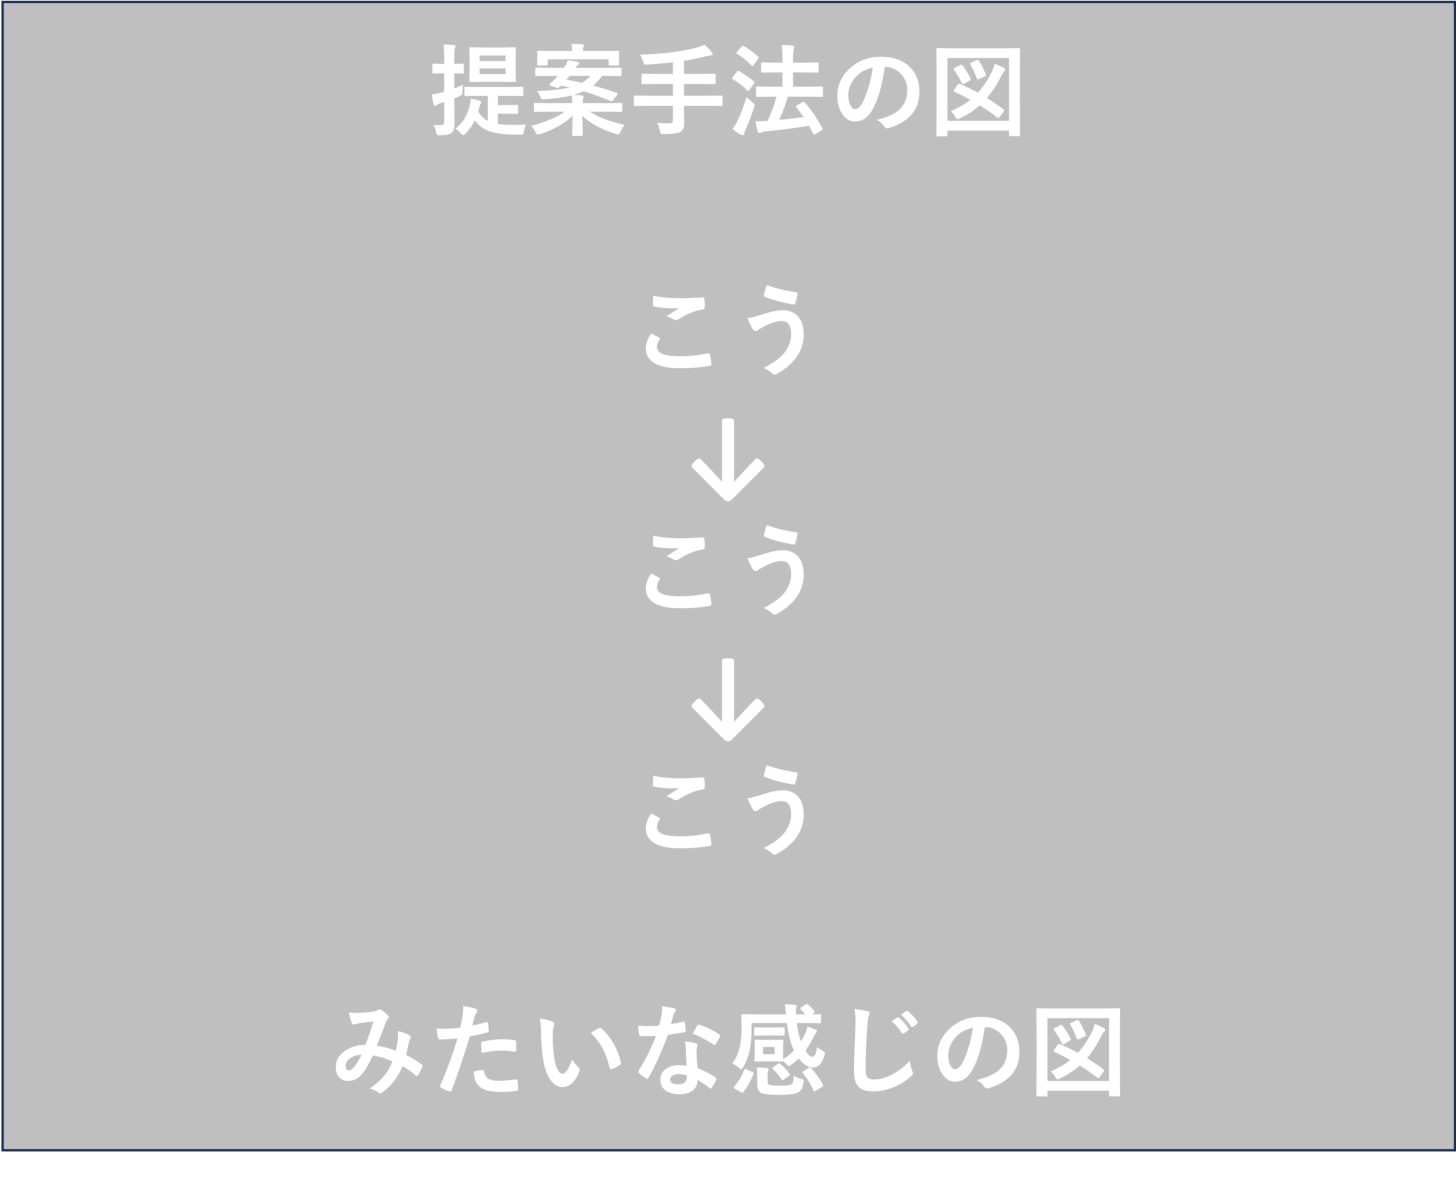
\includegraphics[width=1.0\linewidth]{fig/teiannshuhou.pdf}
  \caption{提案手法の概要}
\end{figure}

提案手法の概要を図\ref{fig:rq2.syuhou}に示す.提案手法の入力は,変更前後の全てのソースファイルであり,出力は後方互換性の有無の予測である.まず,入力として与えられた変更前後の全てのソースファイルから,変更されていないファイルを除外し,テストコードが記述されたファイルを抽出する.テストコードが記述されたファイルの条件は,ファイルパスに{\verb|test|}または{\verb|spec|}を含み,ファイル名の末尾が{\verb|.js|}または{\verb|.ts|}で,{\verb|.d.ts|}を除いたファイルとする.例えば,{\verb|test.js|}や,{\verb|spec/index.ts|}などをテストコードが記述されたファイルとして抽出する.次に,抽出したソースファイルにおける,変更されたプログラム部分とその変更情報を\ref{subsec:rq2.astseisei}章の方法で特定する.最後に,変更されたプログラム部分とその変更情報が\ref{subsec:rq2.jouken}章で述べる3つの条件に1つでも一致すれば,後方互換性が損失したと判定し,どれにも一致しなければ後方互換性を維持していると判定する.

\subsection{変更されたプログラム部分と変更情報の特定}\label{subsec:rq2.astseisei}
変更されたプログラム部分と変更情報の特定のために,抽象構文木(AST)ベースの差分解析ツールであるGumTree\cite{gumtree}を利用する.ASTとは,ソースコードを構文解析して得られる木構造のデータである.GumTreeは,変更前後のソースファイルまたはASTを受け取ると,それらを比較してASTのノード単位の編集操作を出力する.検出できる編集操作は,「削除」「挿入」「移動」「変更」である.ただし,GumTreeはファイル単位の差分しか検出することができず,ファイルを横断するソースコードの移動操作に対して「移動」ではなく「削除と挿入」として出力されてしまう.ファイルを横断するテストコードの移動はリファクタリングにおいて一般的に行われるため誤検出の原因となる.本手法では,藤本らの手法\cite{gumtreenoyatu}を一部利用し,以下の手順で複数ファイルを横断してGumTreeを適用する.

\begin{enumerate}
  \setlength{\itemsep}{0cm}
  \item 変更のある各ファイルごとにASTを生成する
  \item 根となるノードを1つ作成する
  \item 各ファイルごとに生成したASTを子ノードとして加えていく
  \item 1から3を変更前後で実施し,2つASTを生成する
  \item 変更前後で生成された2つのASTをGumTreeに入力して出力を得る
\end{enumerate}

この方法により,バージョン間のテストコード変更に対して,変更されたプログラム部分(ノード)と,「削除」「挿入」「移動」「変更」の4つの変更情報をファイルを横断する移動操作も含めて特定することができる.

\subsection{後方互換性を損失したと判定する条件}\label{subsec:rq2.jouken}
\ref{chap:rq1}章で述べた,「既存のテストスイート内でのテストコード追加」「テストコード削除」「アサーションの入力値と期待値のいずれか一方の変更」を自動で検出するために,それぞれ条件を定義する.

まず,「既存のテストスイート内でのテストコード追加」「テストコード削除」を判定するために,テストコードを定義する.従来研究\cite{matsuda}では,テストファイル内に記述されている,関数名が{\verb|it|}または{\verb|test|}である関数呼び出しをテストケースとしている.本研究では,テストスイートの追加・削除を含めるため,慣習的にテストスイートの宣言として使われる{\verb|describe|}という関数名を加え,{\verb|it|}または{\verb|test|}または{\verb|describe|}という関数呼び出しで,第一引数が文字列,第二引数が関数であるものをテストスイートまたはテストケースと定義する.

次に,「アサーションの入力値と期待値のいずれか一方の変更」を判定するために,アサーションの入力値と期待値を定義する.JavaScript言語では,アサーションの書き方はフレームワークによって異なる.本手法では,State of JavaScript 2022\footnote{\url{https://2022.stateofjs.com/}}で紹介されている主要なテストフレームワーク13件のうち,単体テストで使われるフレームワーク5件(Jest\footnote{\url{https://jestjs.io/}},Mocha\footnote{\url{https://mochajs.org/}},AVA\footnote{\url{https://github.com/avajs/ava}},Jasmine\footnote{\url{https://jasmine.github.io/}},Vitest\footnote{\url{https://vitest.dev/}})を考慮する.Mochaは複数のアサーションの記述スタイルを利用できるため,Mochaで使用可能なアサーションのスタイルについても考慮する.テストフレームワーク毎のアサーションの書き方は,大きく2つに大別できる.例をProgram\ref{bdd.test.js},Program\ref{tdd.test.js}で示す.

\begin{lstlisting}[caption=アサーション例1, label=bdd.test.js]
expect(calculator.add(1, 1)).to.be.a('number').equal(2);
expect(calculator.add(1, 1), 'to be', 2);
calculator.add(1, 1).should.be.a('number').equal(2);
\end{lstlisting}

Program\ref{bdd.test.js}は,自然言語に似た構文を使用してテストを記述する記述形式で,Jest,Mocha,Jasmine,Vitestで使用される.その中でも,1行目のように,{\verb|expect|}関数にメソッドチェーンで振る舞いを記述する形式,2行目のように{\verb|expect|}関数の引数にそのまま振る舞いを記述する形式,3行目のように入力値に{\verb|should|}プロパティを追加して振る舞いを記述する形式がある.1,2行目の形式に対しては,{\verb|expect|}関数の第一引数を入力値,それ以降を期待値として扱い,3行目の形式に対しては,{\verb|should|}プロパティ以前を入力値,以降を期待値として扱う.

\begin{lstlisting}[caption=アサーション例2, label=tdd.test.js]
assert.equal(calculator.add(1, 1), 2);
t.is(calculator.add(1, 1), 2);  
t.true(calculator.add(1, 1) === 2);
\end{lstlisting}

Program\ref{tdd.test.js}は,Node.js\footnote{\url{https://nodejs.org/en}}標準の{\verb|assert|}文がメインの記述形式で,AVA,Mochaで使用される.その中でも,1行目や2行目のように,第一引数に入力値,第二引数に期待値を取る形式と,3行目のように入力だけを引数に取る形式がある.この記述形式に対しては,{\verb|assert|},{\verb|t|},{\verb|test|}をキーとして,アサーションメソッドの第一引数を入力,第二引数を期待値として扱う.3行目のように引数が1つの場合は,引数を入力,アサーションメソッド名を期待値とする.

以上の定義を利用し,後方互換性の損失に伴うテストコード変更内容である,「既存のテストスイート内でのテストコード追加」「テストコード削除」「アサーションの入力値と期待値のいずれか一方の変更」を検出する条件を以下に定める.

\begin{itemize}
  \item \textbf{既存のテストスイート内でのテストコード追加}:GumTreeで「挿入」と判定されたプログラム部分がテストコードまたはアサーションであり,かつ既存のテストコード内で追加されていること
  \item \textbf{テストコード削除}:GumTreeで「削除」と判定されたプログラム部分がテストコードであること
  \item \textbf{アサーションの入力値と期待値のいずれか一方の変更}:GumTreeで「変更」と判定されたノードがアサーションの入力値もしくは期待値であり,同じアサーションの入力値もしくは期待値がGumTreeで「変更」と判定されていないこと
\end{itemize}

ライブラリバージョンに含まれるテストコード変更内容が,以上3つの条件に1つでも当てはまれば,ライブラリバージョンは後方互換性を損失したと判定し,1つも当てはまらなければライブラリバージョンは後方互換性を維持したと判定する.

\section{データセット}
データセットは,\ref{rq1:datasets}章と同様の従来研究\cite{matsuda}で収集されたライブラリバージョン2,111件を使用し,削除や非公開になったことによりGitHub上でアクセスできないものと,GumTree上でエラーになるもの計156件を除いた1,955件を使用する.

\section{分析結果}

データセットに対して,従来手法と,\ref{sec:rq2.teian}章で述べた手法を適用した.結果を表\ref{fig:result}に示す.分析対象とするライブラリバージョン1,955件中,提案手法で後方互換性なしと予測したライブラリバージョンは662件(約34%),後方互換性ありと予測したライブラリバージョンは1,293件(約66%)であった.また,従来手法で後方互換性なしと予測したライブラリバージョンは905件(約46%),後方互換性ありと予測したライブラリバージョンは1,050件(54%)であった.

提案手法で後方互換性を損失したと予測したライブラリバージョン662件中,114件(約17%)は後方互換性を損失し,662件中548件(約83%)は後方互換性を維持している.また,後方互換性を損失したライブラリバージョン223件中,114件(約51%)を正しく予測した.従来手法では,後方互換性を損失したと予測したライブラリバージョン905件中,140件(約15%)が後方互換性を損失し,後方互換性を損失したライブラリバージョン223件中.140件(63%)を正しく予測した.

従来手法で後方互換性なしと判定したライブラリバージョン中765件が誤判定だったのに対し,提案手法では548件が誤検出であった.これは,従来手法で誤検出となる,テストケースの移動やラベルの修正などのテストコードのリファクタリングによる影響を提案手法では受けないため,誤検出を減らすことができたことを示している.一方で,提案手法は従来手法に比べて,後方互換性を損失したライブラリバージョンの検出精度が低下している.従来手法では後方互換性を損失したライブラリバージョン223件中,140件を正確に検出できたのに対し.提案手法では114件のみを検出した.この結果から,提案手法は誤検出を減らすことには成功しているが,後方互換性を損失したライブラリバージョンの検出においては改善の余地があるとわかる.

予測結果を目視により調査した内容については,\ref{rq2:kousatu}章で言及する.

\begin{table}[]
  \centering
  \label{fig:result}
  \begin{tabular}{l|r|r|r}
    \hline
                    & \multicolumn{1}{c|}{後方互換性なし} & \multicolumn{1}{c|}{後方互換性あり} & \multicolumn{1}{c}{合計} \\ \hline
    後方互換性なしと予測      & 114                          & 548                          & 662                    \\ \hline
    後方互換性ありと予測      & 109                          & 1,184                        & 1,293                  \\ \hline
    合計              & 223                          & 1,732                        & 1,955                  \\ \hline\hline
    従来手法で後方互換性なしと予測 & 140                          & 765                          & 905                    \\ \hline
    従来手法で後方互換性ありと予測 & 83                           & 967                          & 1,050                  \\ \hline
    合計              & 223                          & 1,732                        & 1,955                  \\ \hline
  \end{tabular}
\end{table}



\section{考察}\label{rq2:kousatu}
分析したライブラリバージョンを目視で確認し,ライブラリバージョンの例を挙げて分析結果について考察する.

\subsection{従来手法と提案手法の検出性能に関する考察}
後方互換性を損失しているライブラリバージョンで,従来手法では正確に検出できており,提案手法で誤検出した原因について考察する.例として,\todo{〜〜〜}を示す.
% 従来手法のチート
% 正解データの集め方

% テストケー スの削除や修正が行われたが,それに伴って影響を受けるクライアントが存在しなかった原因を 考察する.まず,ライブラリバージョンの後方互換性が維持されていたため,全てのクライアント に影響を与えなかったことが考えられる.例として,値が Stream オブジェクトであることを検証 する関数を提供するライブラリである is-stream のバージョン 1.0.1 から 1.1.0 への変更 1を図 6.1 に示す.


%本研究では、従来の後方互換性判定手法に対して、テストコードの変更内容を詳細に分析することで誤検出を減らす提案手法を開発しました。従来手法が一定の「チート」を行っていると考えられる点に注目しました。具体的には、従来手法では単純にテストコードに変更があれば、それを後方互換性の損失と判定していました。これに対し、本研究の提案手法では、テストコードの変更だけではなく、その変更の性質を考慮に入れることで、より正確な後方互換性の損失の判定を目指しました。

%従来手法のこのアプローチは、テストコードのリファクタリングや無関係の変更によっても後方互換性の損失と誤判定されるリスクがありました。例えば、ライブラリ本体では後方互換性に影響を与える変更がなされていないにもかかわらず、テストコードがリファクタリングされることで後方互換性を損失したと誤判定されるケースです。これは、従来手法がライブラリ本体の変更とテストコードの変更の関連性を十分に評価していないことに起因します。提案手法では、この点を改善し、ライブラリ本体の変更とテストコードの変更の関連性を厳格に評価することで、誤検出の削減を図りました。

%提案手法で後方互換性を損失したと判定する条件を絞り込んだ結果、当然ながら検出件数が減少し、その結果として精度が低下することが観察されました。従来手法では、テストコードの任意の変更を後方互換性の損失の指標としていたため、より多くのライブラリバージョンを後方互換性がないと判定していました。しかし、このアプローチは多くの誤検出をもたらすリスクがあり、実際の後方互換性の状況を正確に反映していない可能性があります。提案手法による精度の低下は、後方互換性を損失したと判定する条件をより現実的なものに絞り込んだ結果と解釈できます。

%また、後方互換性の正確な判定には、実際に使用されているクライアントのテストコードを分析することが重要です。しかし、クライアントのテストが不十分な場合、ライブラリ本体に後方互換性を損失する変更があったとしても、それが検出されずに後方互換性ありと分類されてしまうリスクがあります。この問題は、正解データの質に直接影響を与え、分析の精度を低下させる可能性があります。したがって、正解データをより正確に収集し分析することが、今後の課題として残されています。

\section{まとめ}
本章では,テストコードの変更内容に基づく後方互換性の判定手法の有効性について検証した.提案手法では,従来手法と比較して,テストコードの変更内容を詳細に分析することで,後方互換性の損失をより正確に予測することを目指した.

分析結果から,提案手法は従来手法に比べて,後方互換性を維持しているライブラリバージョンに対し,後方互換性を損失したと誤検出する件数を減らすことができた.一方で,後方互換性を損失したライブラリバージョンの検出においては,提案手法の精度が従来手法の精度より低下していることがわかった.これは,提案手法が後方互換性を損失したと判定する条件を絞ったため,検出件数が減少し,結果として精度が低くなったと考えられる.

また,後方互換性の判定精度の検証には,クライアントのテストコードの分析が重要であると再確認された.不十分なクライアントのテストコードは,正解データの質に影響を与え,分析の精度を低下させるため,今後の研究では正解データをより正確に収集し分析することが求められる.


\chapter{妥当性への脅威}\label{chap:heuristic}

\section{内的妥当性}

\section{外的妥当性}

\chapter{おわりに}\label{chap:end}

\chapter*{謝辞}

本研究を進めるにあたって,多くの方々に,御指導,御協力,御支援を賜りました.ここにお世話になった方々への感謝の意を記させていただきます.



% 文献を参照する場合には,論文の最後に参考文献として列挙するとともに,
% \verb|\cite|を使って,例えば,
% \begin{quote}
%   文献\cite{1390850475731067264}によれば…
% \end{quote}
% や,
% \begin{quote}
%   …である\cite{latex2e}.
% \end{quote}
% のように参照する.

% 文献の列挙には,{\tt thebibliography}環境などを用いる\footnote{使い方
%   は,この資料のソースを参照.}.

%%%%%%%%%%%%%%%%%%%%%%%%%%%%%%%%%%%%%%%%%%%%%%%%%%%%%%%%%%%%%%%%%%%%%%%%

%%
%% 謝辞
%%
%% \begin{acknowledgements}
%% 感謝します.
%% \end{acknowledgements}

%%%%%%%%%%%%%%%%%%%%%%%%%%%%%%%%%%%%%%%%%%%%%%%%%%%%%%%%%%%%%%%%%%%%%%%%

%%
%% 参考文献
%%

\bibliographystyle{junsrt}
\bibliography{thesis}

%%%%%%%%%%%%%%%%%%%%%%%%%%%%%%%%%%%%%%%%%%%%%%%%%%%%%%%%%%%%%%%%%%%%%%%%

%%
%% 付録
%%
% \appendix
% 
% \chapter{サンプルプログラム}
% 
% プログラムリストや実行結果など,本論を補足する上で必要と思われるものが
% あれば付録として付ける.
% 
% {
% \footnotesize
% \begin{verbatim}
% #include <stdio.h>
% int main(void)
% {
%     printf("Hello, World!\n");
%     return 0;
% }
% \end{verbatim}
% }

%%%%%%%%%%%%%%%%%%%%%%%%%%%%%%%%%%%%%%%%%%%%%%%%%%%%%%%%%%%%%%%%%%%%%%%%

\end{document}
